\documentclass[12pt,a4paper]{report}

\usepackage[utf8]{inputenc}
\usepackage[T1]{fontenc}
\usepackage[italian]{babel}
\usepackage[margin=2.5cm]{geometry}
\usepackage{graphicx}
\graphicspath{{images/}{./}}
\usepackage[hidelinks]{hyperref}
\usepackage{xcolor}
\usepackage{listings}
\usepackage{xltabular}
\usepackage{booktabs}
\usepackage{enumitem}
\usepackage[table]{xcolor}
\usepackage{float}
\usepackage{hyperref}
\usepackage[normalem]{ulem}

\lstset{
    basicstyle=\ttfamily\small,
    keywordstyle=\color{blue}\bfseries,
    commentstyle=\color{green!60!black},
    stringstyle=\color{red},
    showstringspaces=false,
    breaklines=true,
    frame=single,
    rulecolor=\color{black!30},
    literate={€}{{\texteuro}}1
}

% Stile per i listati dei test: numerazione delle righe come nei code snippet
\lstdefinestyle{testcode}{
    numbers=left,
    numberstyle=\tiny\color{black!45},
    numbersep=8pt,
    xleftmargin=2.2em,
    captionpos=t
}
\begin{document}

\begin{titlepage}
    \centering
    
    % LOGO
    
\includegraphics[width=0.4\textwidth]{logo_unifi.png}\par
    \vspace{0.5cm}
    
    % INTESTAZIONE
    {\Large \textsc{Università degli Studi di Firenze} \par}
    {\large Scuola di Ingegneria \par}
    {\small Corso di Laurea in Ingegneria Informatica \par}
    \vspace{1.5cm}
    
    % TITOLO
    \rule{\linewidth}{0.3mm} \par
    \vspace{0.8cm}
    {\huge \textbf{ChargeNet} \par}
    \vspace{0.3cm}
    {\Large \textit{Piattaforma per la gestione di stazioni di ricarica per veicoli elettrici} \par}
    \vspace{0.6cm}
    \rule{\linewidth}{0.3mm} \par
    \vspace{1cm}

    \href{https://github.com/TommasoSottili/ChargeNet}{\colorbox{black}{\textcolor{white}{\Large\textbf{\ \ Repository GitHub\ \ }}}}

    \vspace{1.5cm}

    \begin{minipage}[t]{0.45\textwidth}
        \begin{flushleft} \large
            \textbf{Candidati:}\\
            Tommaso Sottili 7138541\\
            Luca Moracci 7140812\\
            Marco Lampronti 7147400
        \end{flushleft}
    \end{minipage}
    \hfill
    \begin{minipage}[t]{0.45\textwidth}
        \begin{flushright} \large
            \textbf{Corso:}\\
            Ingegneria del software\\
            \textbf{Docente:}\\
            Prof. Enrico Vicario
        \end{flushright}
    \end{minipage} 
    
    \vfill 
    
    {\large Anno Accademico 2025/2026 \par}
    
\end{titlepage} 

% INDICE 
\tableofcontents
\clearpage

\chapter{Introduzione}


\section{Descrizione}
Il progetto \textbf{ChargeNet} è un sistema software pensato per la gestione di una rete di stazioni di ricarica per veicoli elettrici (EV). L'idea alla base dell'applicazione è quella di coordinare tutto ciò che ruota attorno a una sessione di ricarica: dall'aiutare l'utente a trovare una colonnina libera, fino alla gestione del pagamento, assicurandosi allo stesso tempo che l'infrastruttura elettrica non subisca danni.

Per raggiungere questo obiettivo, la piattaforma fa da punto di incontro per tre specifiche figure, fornendo a ciascuna le funzionalità necessarie:

\begin{itemize}
    \item \textbf{Driver:} È l'utente finale. Utilizza il sistema per cercare le stazioni compatibili con la sua auto, far partire e monitorare la ricarica, e gestire i pagamenti tramite un portafoglio virtuale interno (wallet).
    
    \item \textbf{Station Operator:} È l'addetto alla manutenzione fisica. Il suo compito è controllare lo stato di salute delle colonnine: se una stazione si guasta, può metterla temporaneamente fuori servizio per evitare disagi ai Driver, e registrarla di nuovo come attiva una volta riparata.
    
    \item \textbf{Energy Manager:} È il tecnico supervisore della rete elettrica. Controlla in tempo reale il carico sui trasformatori per evitare surriscaldamenti. Se la rete è sotto stress, ha gli strumenti per abbassare la potenza erogata o limitare le ricariche (Load Balancing) in modo da proteggere l'infrastruttura.
\end{itemize}

\section{Stack Tecnologico}
Per lo sviluppo è stato scelto un ecosistema Java-centrico, privilegiando 
la robustezza e la portabilità:

\begin{itemize}
    \item \textbf{Linguaggio:} Java 21.
    \item \textbf{Interfaccia Grafica:} JavaFX 21, per una gestione 
    reattiva delle dashboard dei vari attori.
    \item \textbf{Persistenza:} PostgreSQL, gestito tramite JDBC per un 
    controllo granulare delle transazioni.
    \item \textbf{Build Tool:} Maven, per la gestione delle dipendenze e 
    del ciclo di vita del software.
\end{itemize}

\section{Astrazione dell'Infrastruttura Fisica}
Trattandosi di un progetto universitario, l'applicazione non comunica con colonnine e trasformatori reali. Nel mondo reale, infatti, interfacciarsi con l'hardware fisico è un'operazione che porta con sé diverse complicazioni: bisogna gestire le differenze tra i vari produttori, adattarsi a protocolli di rete specifici e gestire i fisiologici ritardi o cadute di connessione dei sensori.

L'architettura del sistema è stata comunque pensata per un'eventuale integrazione futura. Per le finalità di questo progetto, i dati sui consumi e sullo stato delle stazioni vengono semplicemente simulati da un componente interno al programma (\textit{GridMonitor}). 
\chapter{Analisi dei Requisiti e Casi d'uso}

Questo capitolo descrive il processo di progettazione del sistema, seguendo un approccio che va dall'esterno verso l'interno. Si parte dall'analisi di come gli utenti interagiscono con l'applicazione, definendo i requisiti e l'interfaccia grafica, per poi scendere progressivamente nei dettagli tecnici dell'architettura software e della struttura del database.

\section{Use Case Diagram}
Il diagramma dei casi d'uso offre una visione d'insieme delle funzionalità del sistema. Serve a mappare visivamente quali azioni possono compiere i tre attori principali (Driver, Station Operator ed Energy Manager) all'interno della piattaforma.

\begin{figure}[H]
    \centering
    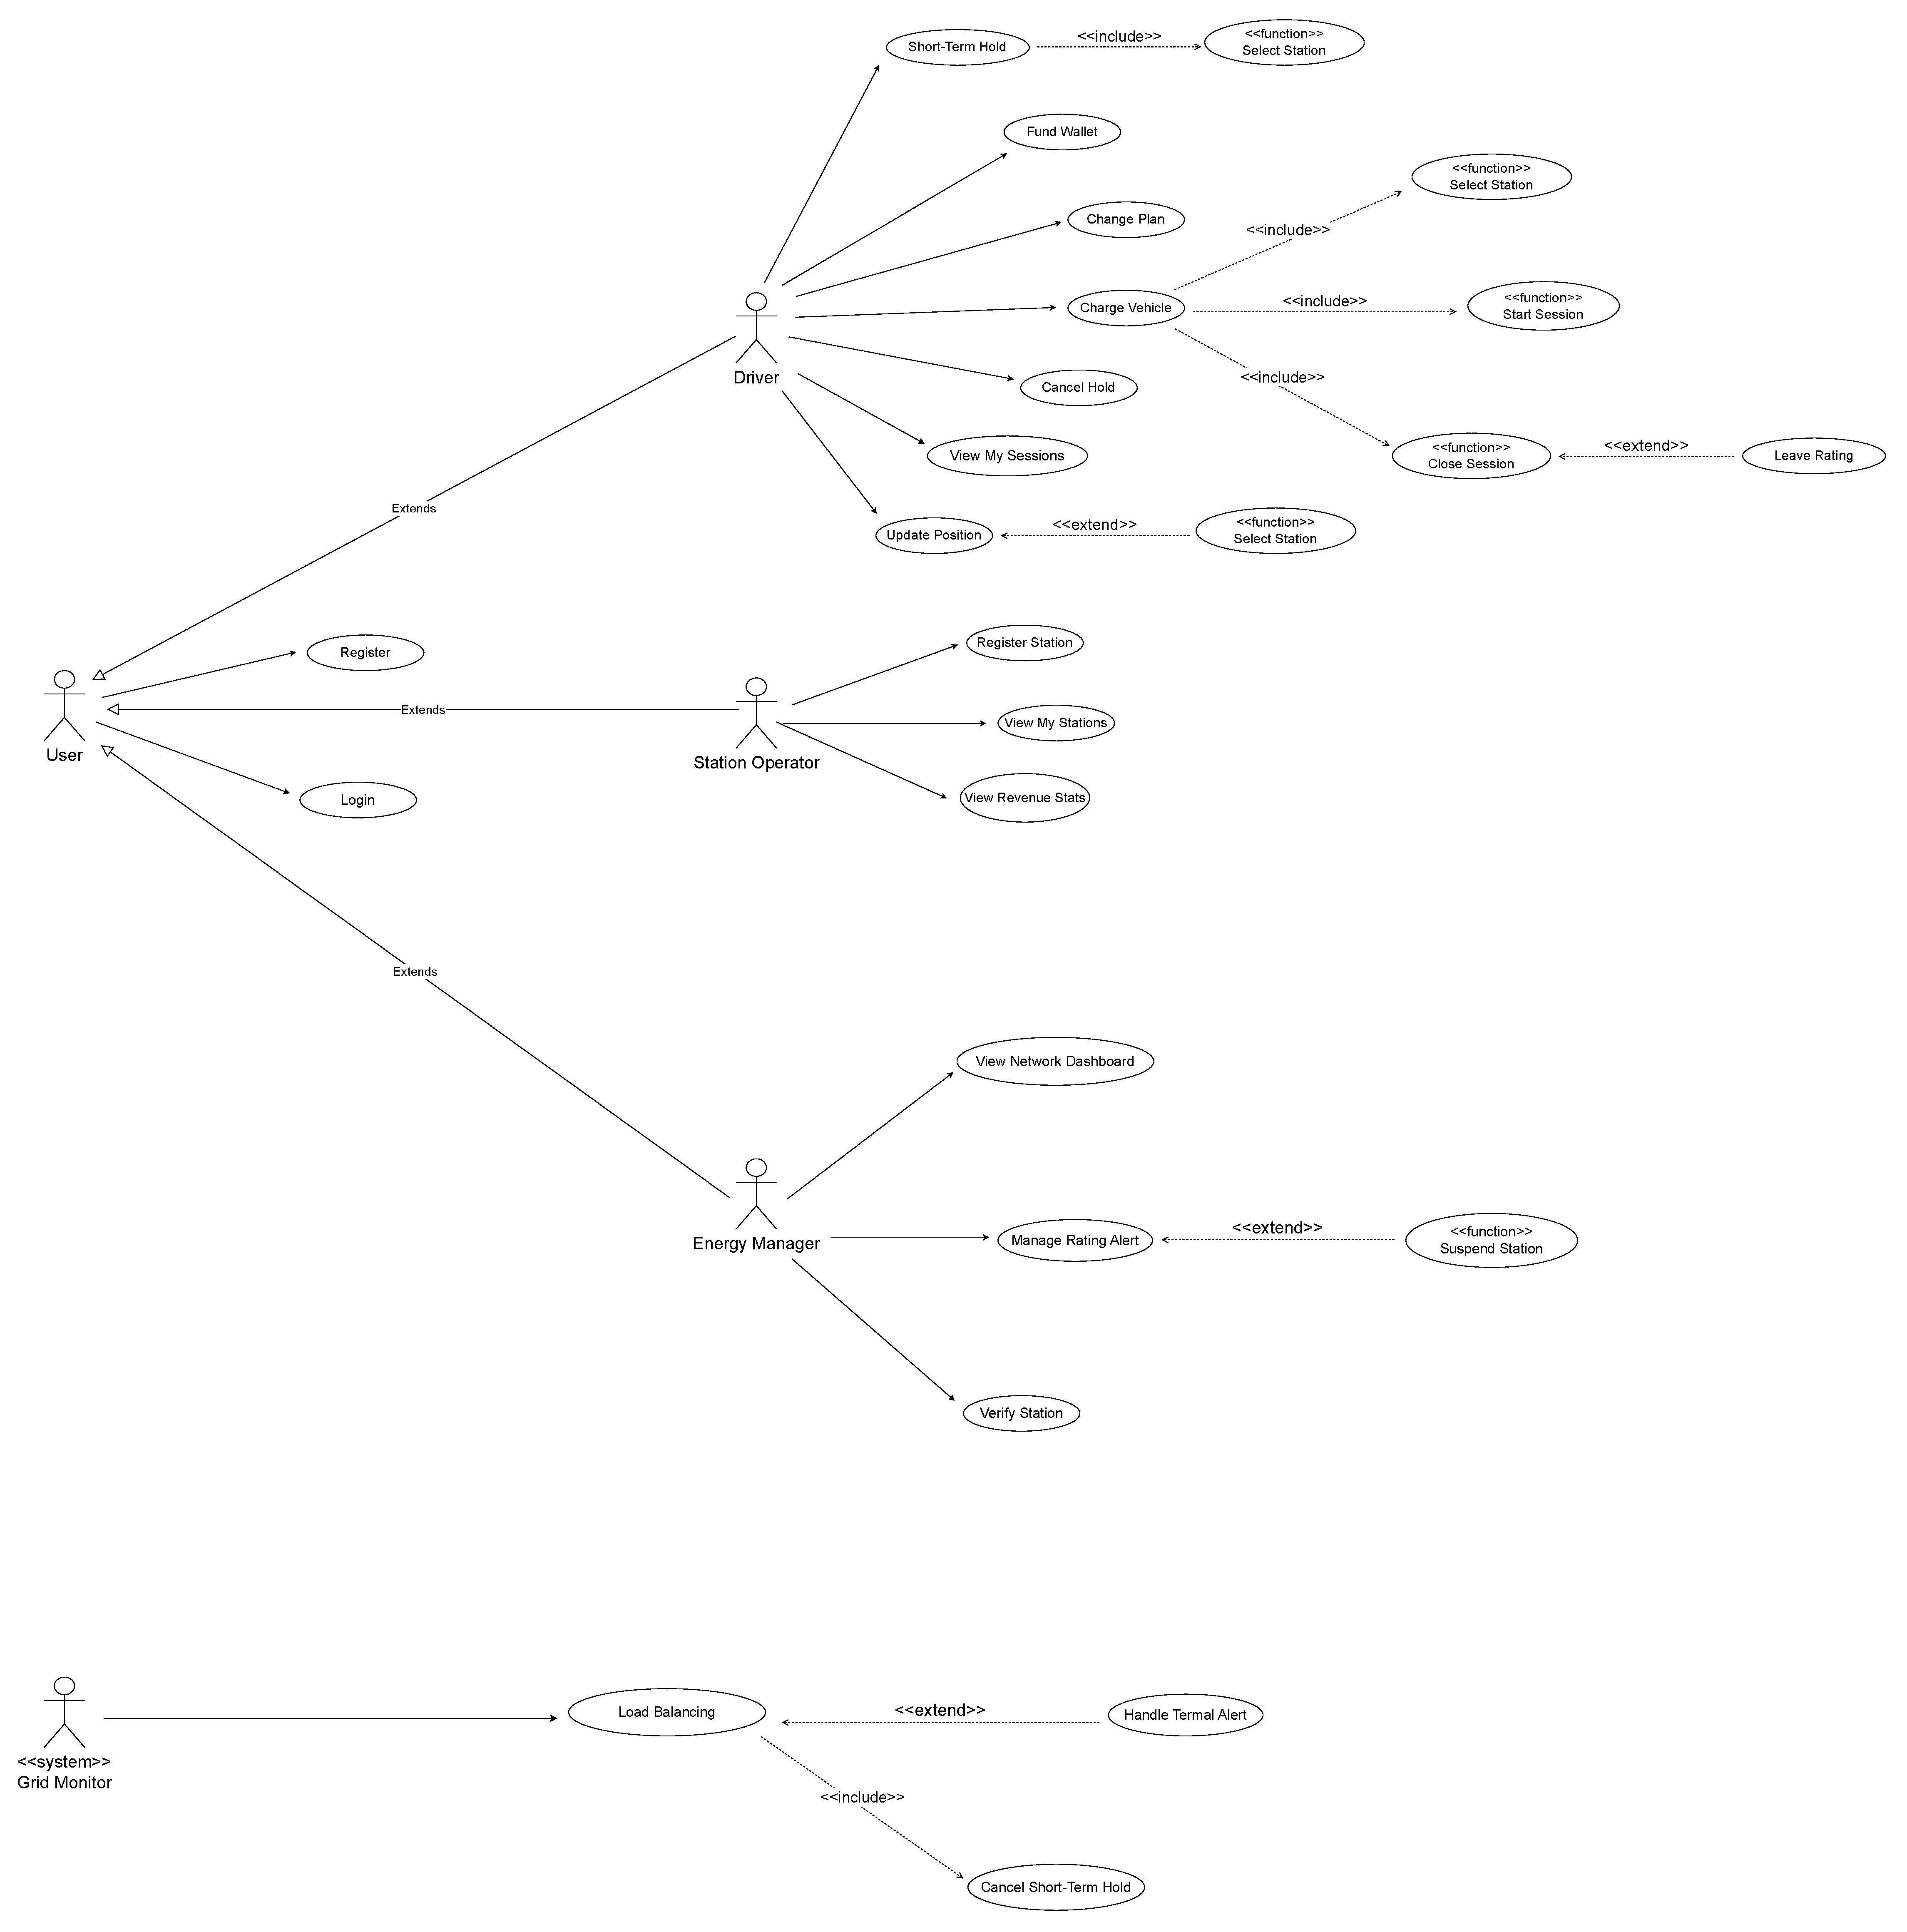
\includegraphics[width=\textwidth]{UseCaseDiagramNew.pdf.drawio.pdf}
    \caption{Diagramma dei casi d'uso}
    \label{fig:mio_schema}
\end{figure}

\section{Use Case Templates}
Per evitare ambiguità, i casi d'uso più importanti sono stati documentati nel dettaglio attraverso dei template strutturati. Questi schemi descrivono passo dopo passo il flusso degli eventi, le precondizioni necessarie e i possibili scenari di errore.
\begingroup
\renewcommand{\arraystretch}{1.4}
\begin{xltabular}{\textwidth}{| >{\bfseries}l | X |}

% --- INTESTAZIONE PRIMA PAGINA ---
\caption{Caso d'Uso: Ricarica Veicolo} \label{tab:uc_ricarica} \\
\hline
\rowcolor{gray!15} Campo & \textbf{Contenuto} \\ \hline
\endfirsthead

% --- INTESTAZIONE PAGINE SUCCESSIVE ---
\multicolumn{2}{c}{{\tablename\ \thetable{} -- Continua dalla pagina precedente}} \\
\hline
\rowcolor{gray!15} Campo & \textbf{Contenuto} \\ \hline
\endhead

% --- PIÈ DI PAGINA (se si spezza) ---
\hline
\multicolumn{2}{r}{\textit{Continua nella pagina successiva...}} \\
\endfoot

% --- PIÈ DI PAGINA FINALE ---
\endlastfoot

% --- CONTENUTO ---
Nome & Ricarica Veicolo (Charge Vehicle) \\ \hline
Livello & Obiettivo Utente (User Goal) \\ \hline
Descrizione & Il Conducente avvia una sessione di ricarica su una stazione selezionata, scegliendo una specifica strategia di ricarica (Fast o Eco). La sessione viene eseguita in tempo reale: il Grid Monitor la fa avanzare e l'interfaccia utente (Live Session UI) ne osserva lo stato tramite polling. \\ \hline
Pre-condizioni & \parbox[t]{\linewidth}{%
Il Conducente ha effettuato l'accesso.\\
Il saldo del Portafoglio (Wallet) del Conducente copre almeno il costo di 5 kWh presso la stazione selezionata, calcolato per il piano del Conducente (\texttt{station.priceFor(5.0, driver)}) e la strategia selezionata.\\
La stazione selezionata è \texttt{ACTIVE} (oppure \texttt{RESERVED} dal Conducente) ed è compatibile con il connettore del veicolo.
} \\ \hline
Post-condizioni & La sessione è \texttt{COMPLETED}, il costo (detratto in modo incrementale per ogni tick durante la ricarica) è interamente addebitato sul Portafoglio, viene registrata una Transazione di tipo \texttt{CHARGE} e la stazione torna allo stato \texttt{ACTIVE}. \\ \hline
Attori & Conducente, Grid Monitor (Sistema) \\ \hline
Unit Test & \texttt{SessionServiceTest} \\ \hline
Flusso Principale & 
\begin{enumerate}[leftmargin=*, nosep]
    \item Il Conducente seleziona una stazione dalla lista delle stazioni disponibili e compatibili più vicine (\texttt{ACTIVE}, o \texttt{RESERVED} da lui stesso).
    \item Il Conducente apre la Live Session per quella stazione.
    \item Il Conducente sceglie una strategia di ricarica: Fast Charge o Eco Charge.
    \item Il Conducente inserisce la percentuale di batteria attuale del veicolo.
    \item Il Conducente preme Start; il sistema valida il saldo del Portafoglio e la disponibilità della stazione, imposta la stazione su \texttt{BUSY} e apre la sessione.
    \item Il Grid Monitor, ogni 5s, aggiorna batteria e kWh erogati, accumula il calore sul trasformatore di alimentazione e deduce i fondi in base alla strategia (lo sconto del piano si applica solo alla quota tariffaria della piattaforma).
    \item La Live Session UI interroga (poll) lo stato della sessione e riflette in tempo reale batteria, kWh, costo attuale e Portafoglio.
    \item Il Conducente preme Stop (oppure la sessione si auto-completa quando la batteria raggiunge il 100\%).
    \item Il sistema calcola i kWh totali erogati, il costo finale e registra la Transazione.
    \item Il sistema reimposta lo stato della stazione su \texttt{ACTIVE} e mostra il popup di valutazione (rating).
\end{enumerate} \\ \hline
Flussi Alternativi & 
\textbf{1. Stazioni non disponibili nascoste:} \newline
1.1. Le stazioni \texttt{BUSY}, \texttt{OVERLOADED}, incompatibili o \texttt{RESERVED} da altri non sono mostrate in lista, impedendo al Conducente di selezionare una stazione non disponibile. \newline\newline
\textbf{5. Saldo insufficiente:} \newline
5.1. Se il saldo è inferiore al costo di 5 kWh, il sistema nega l'avvio e mostra: "Credito insufficiente per avviare la sessione." (\texttt{InsufficientBalanceException}). \newline\newline
\textbf{6-7. Allarme Termico (Observer attivato):} \newline
6.1. Se la temperatura del trasformatore supera i 90°C, il \texttt{LoadBalancerService} (Observer) imposta tutte le stazioni su quel trasformatore su \texttt{OVERLOADED} e chiude forzatamente le relative sessioni attive. \newline
6.2. La sessione diventa \texttt{INTERRUPTED\_THERMAL} e la UI mostra: "Arresto di emergenza: surriscaldamento del sistema". \newline
6.3. Il sistema elabora un rimborso automatico per i kWh pagati ma non erogati. \\ \hline

\end{xltabular} 
\endgroup

\begingroup
\renewcommand{\arraystretch}{1.4}
\begin{xltabular}{\textwidth}{| >{\bfseries}l | X |}

% --- INTESTAZIONE PRIMA PAGINA ---
\caption{Caso d'Uso: Prenotazione a Breve Termine} \label{tab:uc_prenotazione} \\
\hline
\rowcolor{gray!15} Campo & \textbf{Contenuto} \\ \hline
\endfirsthead

% --- INTESTAZIONE PAGINE SUCCESSIVE ---
\multicolumn{2}{c}{{\tablename\ \thetable{} -- Continua dalla pagina precedente}} \\
\hline
\rowcolor{gray!15} Campo & \textbf{Contenuto} \\ \hline
\endhead

% --- PIÈ DI PAGINA (se si spezza) ---
\hline
\multicolumn{2}{r}{\textit{Continua nella pagina successiva...}} \\
\endfoot

% --- PIÈ DI PAGINA FINALE ---
\endlastfoot

% --- CONTENUTO ---
Nome & Prenotazione a Breve Termine \\ \hline
Livello & Obiettivo Utente \\ \hline
Descrizione & Il Conducente riserva per 15 minuti una colonnina \texttt{ACTIVE}, per assicurarsene la disponibilità al proprio arrivo. \\ \hline
Pre-condizioni & \parbox[t]{\linewidth}{%
Il Conducente ha effettuato l'accesso.\\
Non ha già un'altra prenotazione attiva.\\
La colonnina scelta è \texttt{ACTIVE} ed è compatibile con il connettore del veicolo.
} \\ \hline
Post-condizioni & La colonnina è in stato \texttt{RESERVED}, il campo \texttt{reserved\_by\_id} punta al Conducente e \texttt{expiration\_timestamp} è impostato a 15 minuti dall'istante corrente. La colonnina resta visibile al solo Conducente che l'ha prenotata. \\ \hline
Attori & Conducente \\ \hline
Unit Test & \texttt{StationServiceTest} \\ \hline
Flusso Principale &
\begin{enumerate}[leftmargin=*, nosep]
    \item Il Conducente seleziona una colonnina \texttt{ACTIVE} dall'elenco di quelle disponibili.
    \item Conferma di volerla prenotare.
    \item Il sistema tenta l'acquisizione con un \texttt{UPDATE} condizionale, che modifica la riga solo se la colonnina risulta ancora \texttt{ACTIVE}.
    \item Il sistema porta la colonnina a \texttt{RESERVED} e ne registra il Conducente come titolare.
    \item Il sistema imposta \texttt{expiration\_timestamp} a 15 minuti dall'istante corrente.
    \item Il sistema conferma la prenotazione mostrando l'orario esatto di scadenza.
\end{enumerate} \\ \hline
Flussi Alternativi &
\textbf{3. Colonnina non più disponibile:} \newline
3.1. Se nel frattempo un altro Conducente l'ha prenotata o occupata, l'\texttt{UPDATE} non aggiorna alcuna riga e il sistema nega la prenotazione. \newline
3.2. La transazione viene annullata con un \texttt{rollback} e l'oggetto in memoria non viene modificato, così che memoria e database non divergano. \newline
3.3. Il sistema mostra il messaggio \textit{"La colonnina non è più disponibile"} e si torna al passo 1. \newline\newline
\textbf{Nota sulla concorrenza:} \newline
\textbullet\ È il database stesso a impedire la doppia prenotazione: la condizione sullo stato \texttt{ACTIVE} è parte dell'\texttt{UPDATE}, quindi fra due Conducenti simultanei ne può vincere uno solo, senza alcun blocco applicativo. \newline\newline
\textbf{Nota sulla scadenza:} \newline
\textbullet\ Se i 15 minuti trascorrono senza che venga avviata una sessione, il \texttt{GridMonitor} riporta la colonnina ad \texttt{ACTIVE} (Tab.~\ref{tab:uc_update_state}). \\ \hline

\end{xltabular}
 
\endgroup

\section{Mockups}
In questa fase sono stati realizzati i mockup dell'interfaccia grafica per verificare la User Experience e garantire
che tutte le funzionalità descritte nei casi d'uso siano accessibili in modo immediato ed intuitivo.

\section{Page Navigation Diagram}
Il diagramma di navigazione illustra in che modo le diverse schermate dell'applicazione sono collegate tra loro. Mostra il percorso che l'utente compie muovendosi all'interno del sistema in base alle scelte effettuate o ai pulsanti premuti.

\begin{figure}[H]
    \centering
    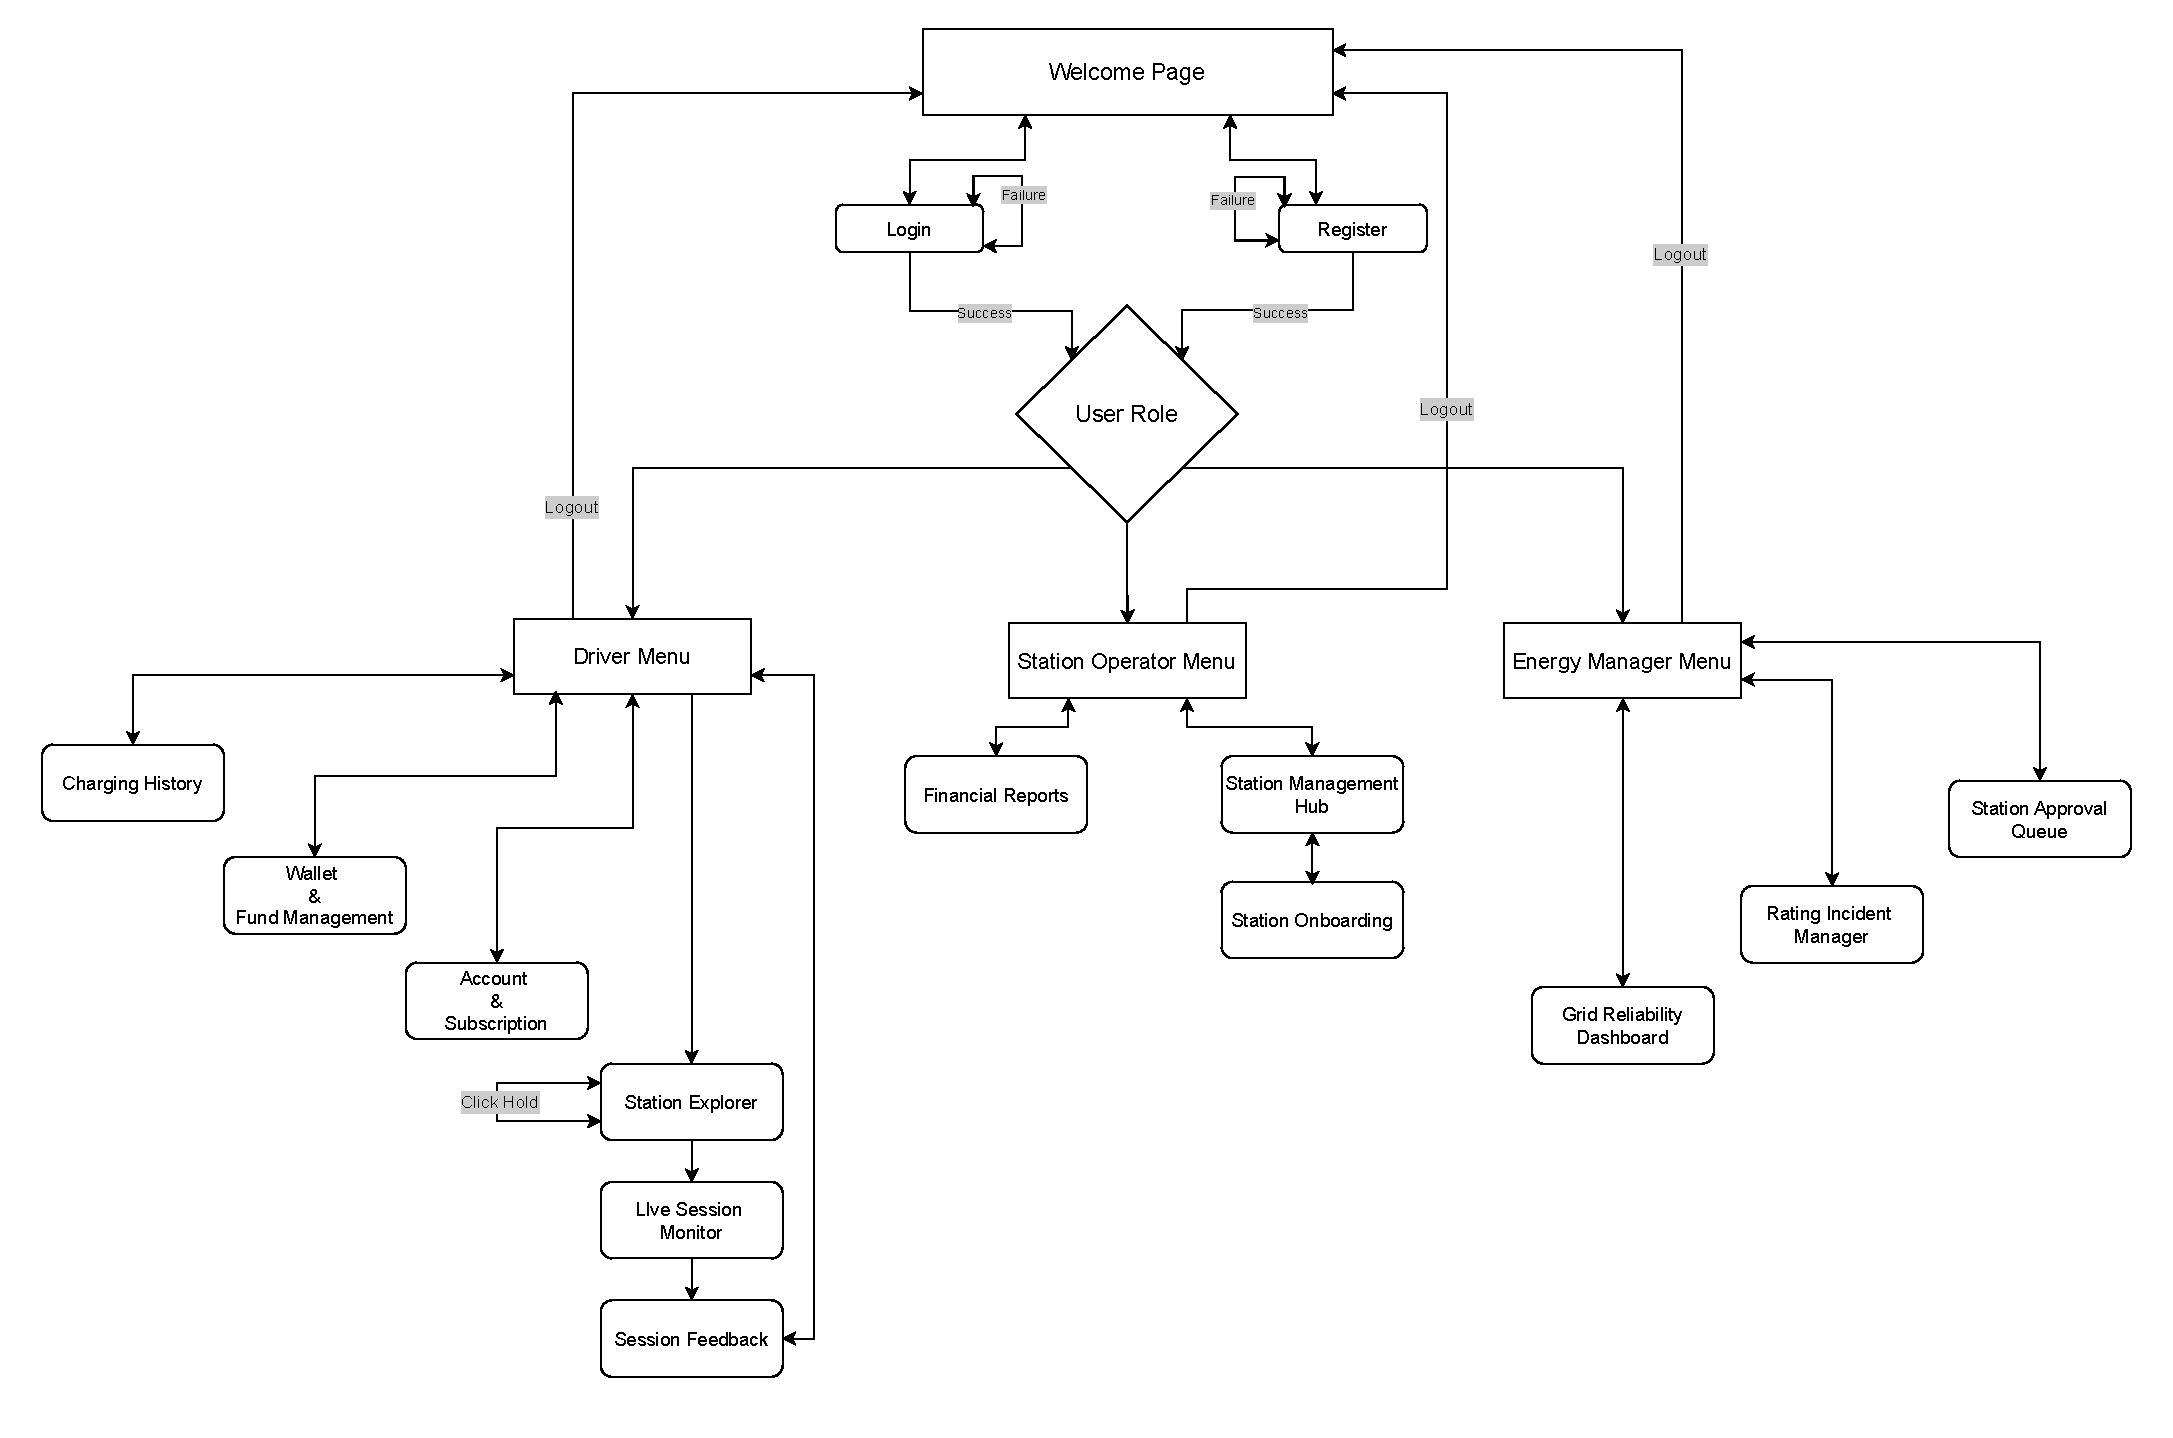
\includegraphics[width=\textwidth]{NavigationPageDiagram.drawio2.pdf}
    \caption{Diagramma di navigazione tra le pagine dell'applicazione.}
    \label{fig:navigation_schema}
\end{figure}

\section{Package Diagram}
Passando all'architettura interna del software, il diagramma dei pacchetti mostra come il codice è stato diviso in moduli logici (come ad esempio la logica di business, l'interfaccia e l'accesso ai dati). L'obiettivo è mantenere il progetto ordinato e limitare le dipendenze tra i vari componenti.

\section{Class Diagram}
Il sistema è stato progettato con un'architettura a strati per mantenere alta coesione e basso accoppiamento (\textit{high coesion and low coupling}). Nel seguente paragrafo sono approfondite le classi principali:

\subsection{Domain Model}

Questo diagramma rappresenta il Domain Model, cioè le entità principali su cui si basa il sistema: utenti, colonnine, trasformatori, sessioni di ricarica e gli oggetti ad esse collegati. Una descrizione più dettagliata sul Domain Model è presente nel paragrafo \ref{sec: Domain Model}

\begin{figure}[H]
    \centering
    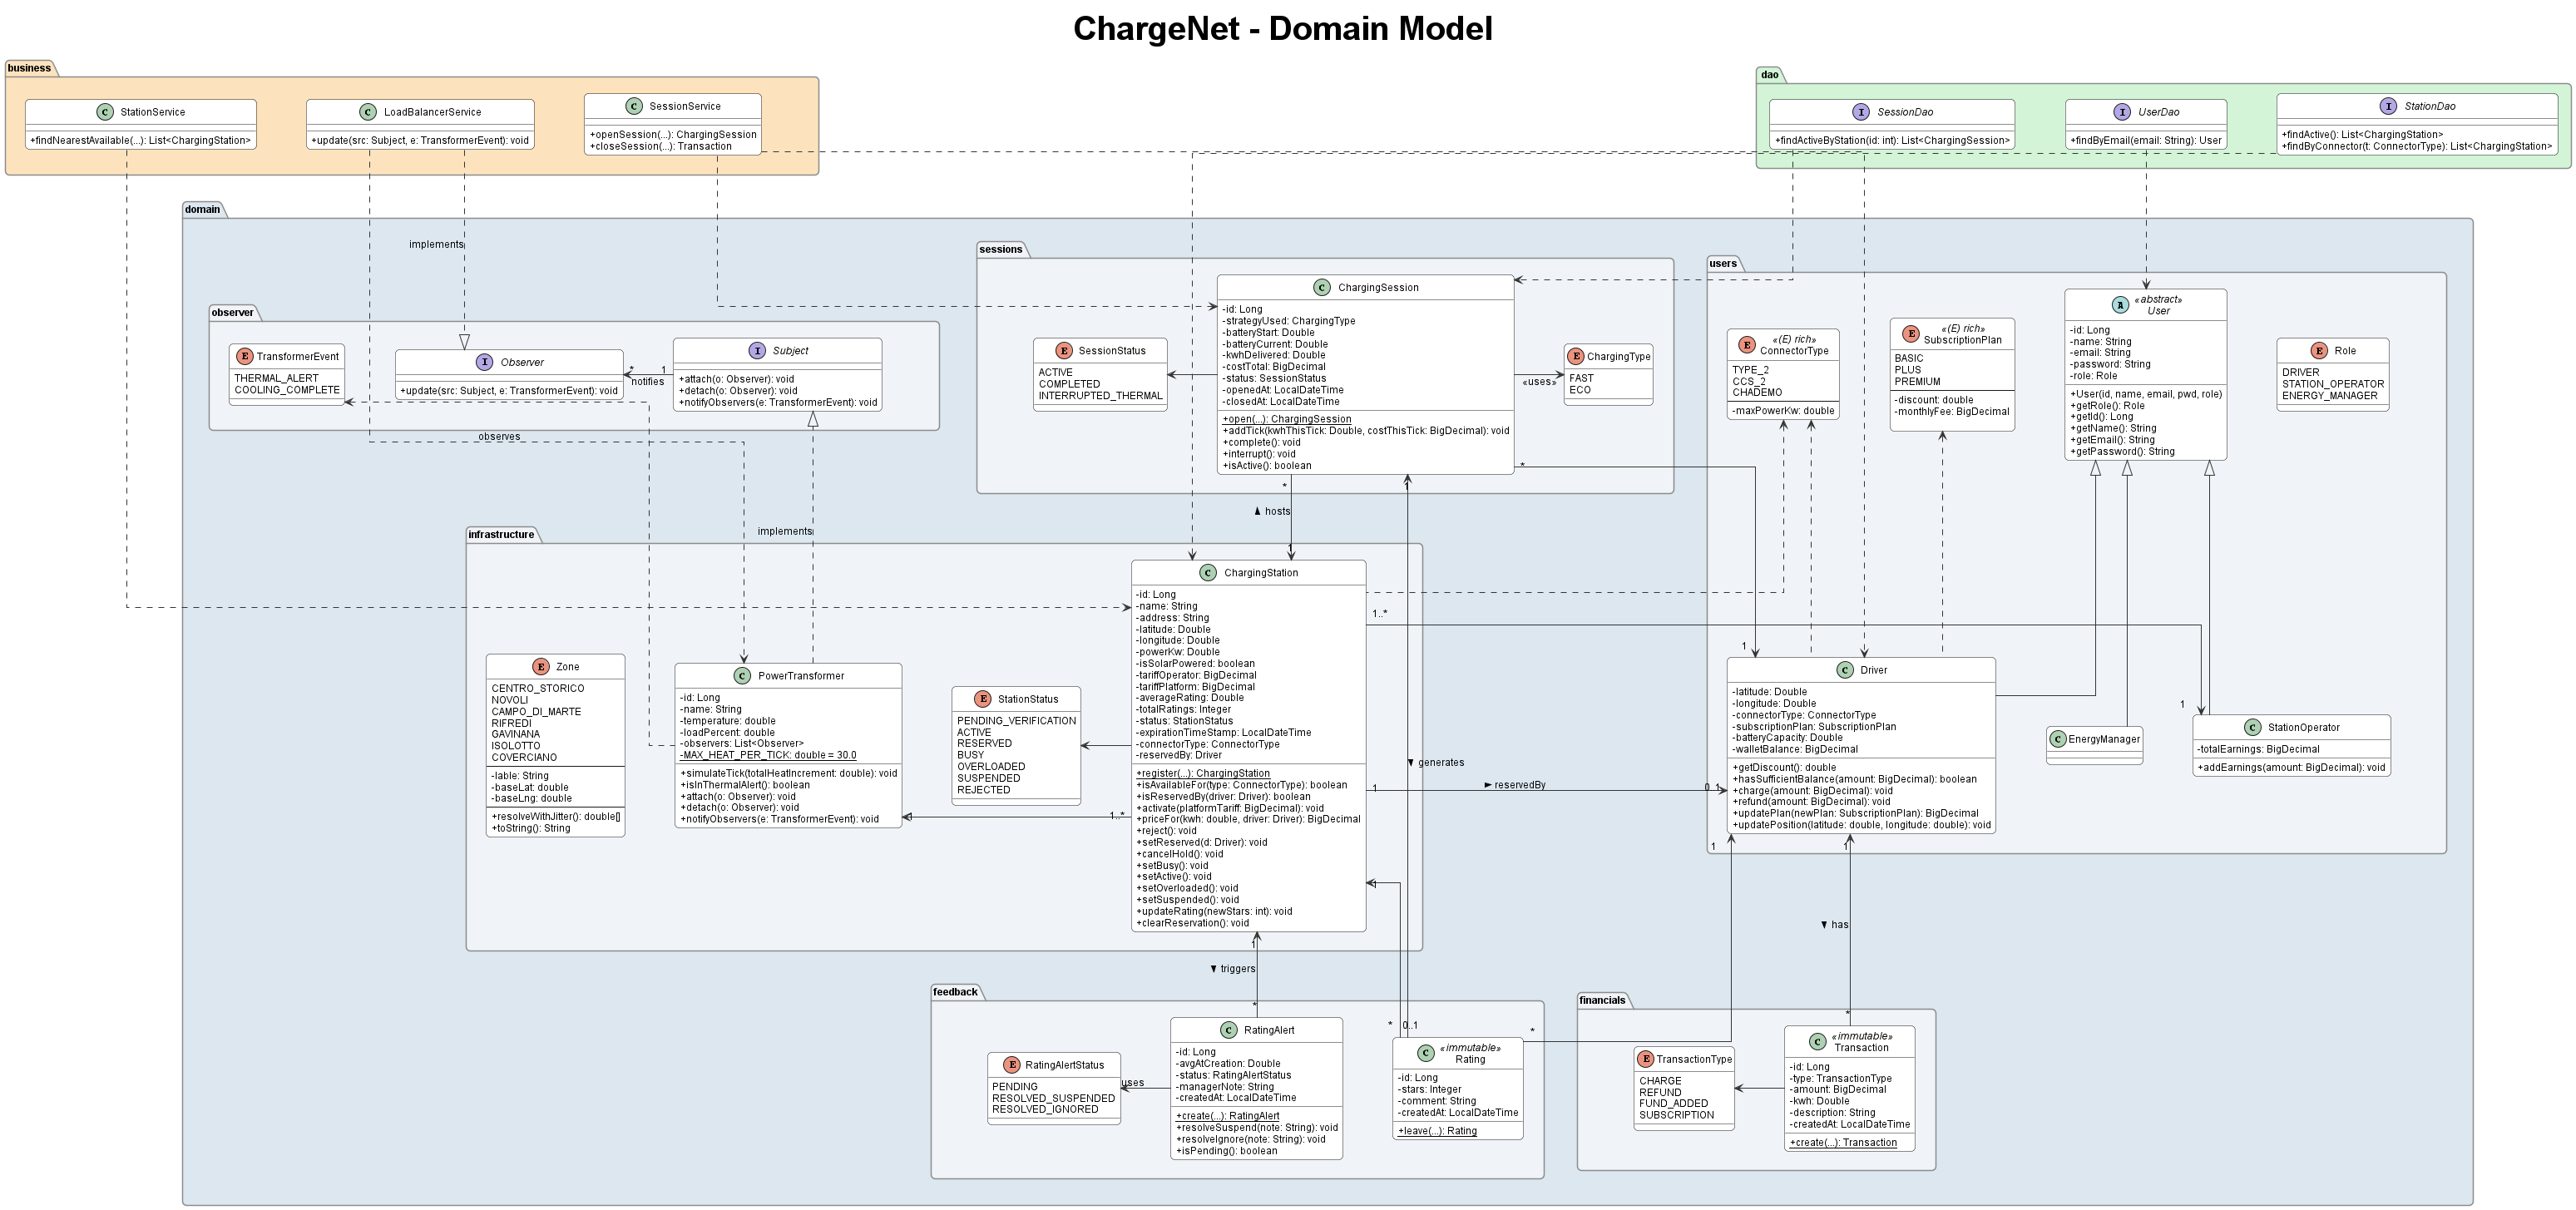
\includegraphics[width=1.10\textwidth]{domain_model.png}
    \caption{Domain Model, diagramma di classe}
    \label{fig:domain_model}
\end{figure}

\subsection{Business Layer}

Il seguente diagramma mostra il Business Layer, il livello che contiene la logica applicativa del sistema. Qui si trovano i servizi che coordinano le entità del Domain Model, le strategie di ricarica e i componenti che gestiscono la simulazione della rete. Il livello è approfondito nel paragrafo \ref{sec: Business}.

\begin{figure}[H]
    \centering
    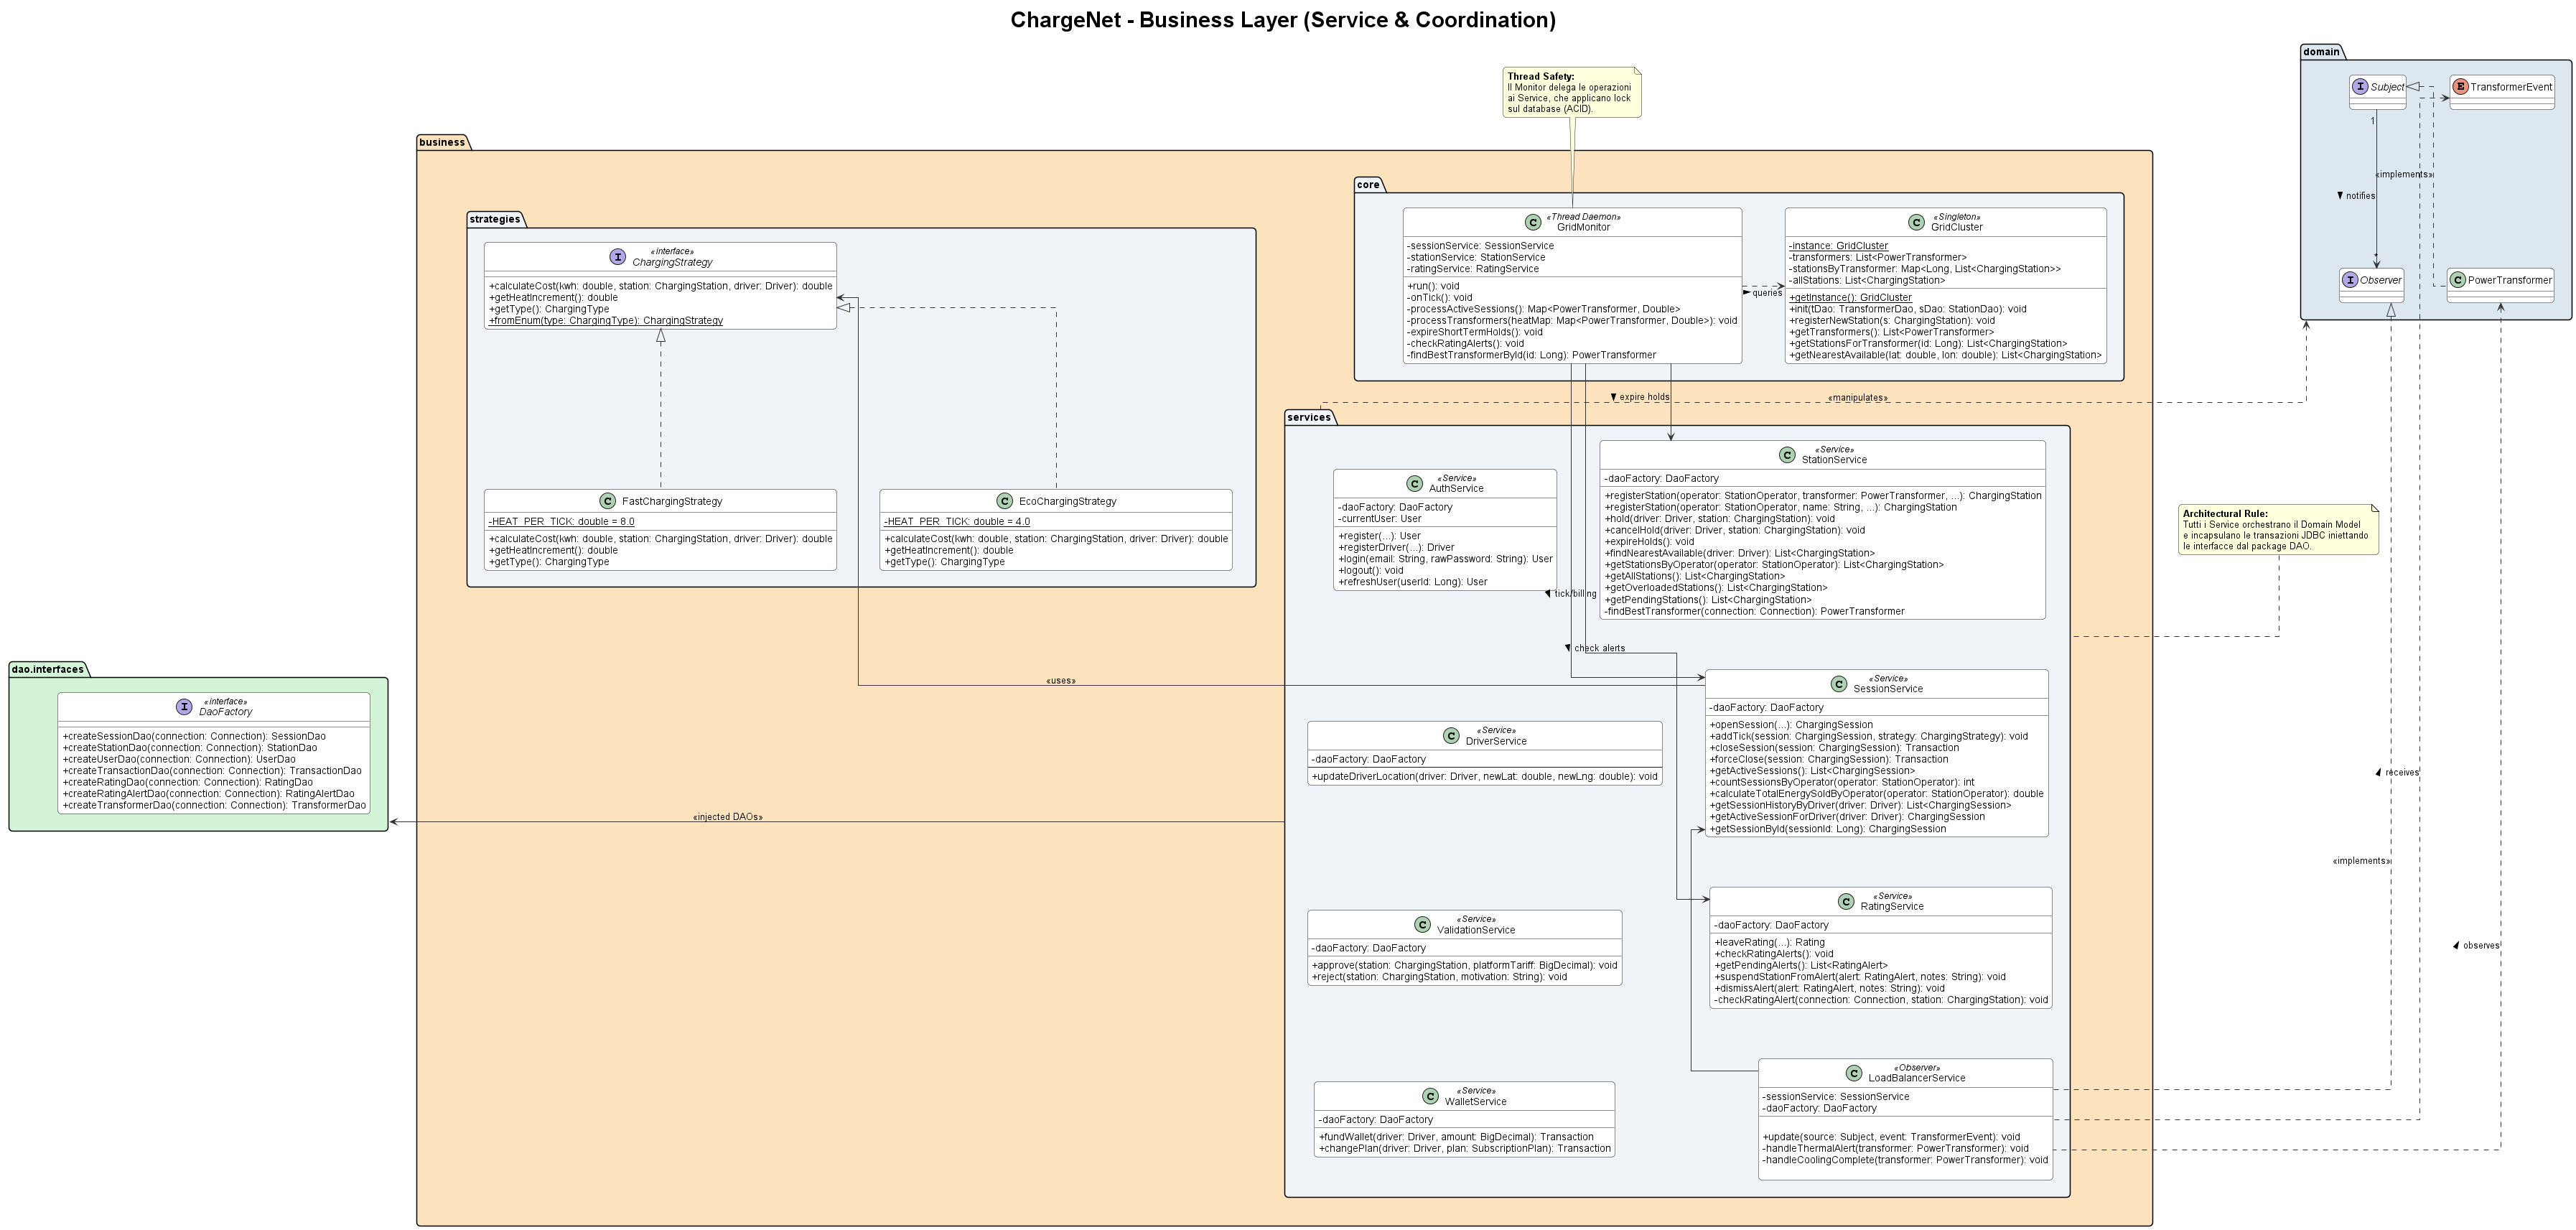
\includegraphics[width=1.10\textwidth]{buiness.png}
    \caption{Business Layer, diagramma di classe}
    \label{fig:business_layer}
\end{figure}

\subsection{DAO}

Di seguito è mostrato il diagramma del livello DAO, responsabile della comunicazione con il database. Il suo compito è tradurre le entità del Domain Model in dati salvabili e recuperabili, garantendone quindi la persistenza

\begin{figure}[H]
    \centering
    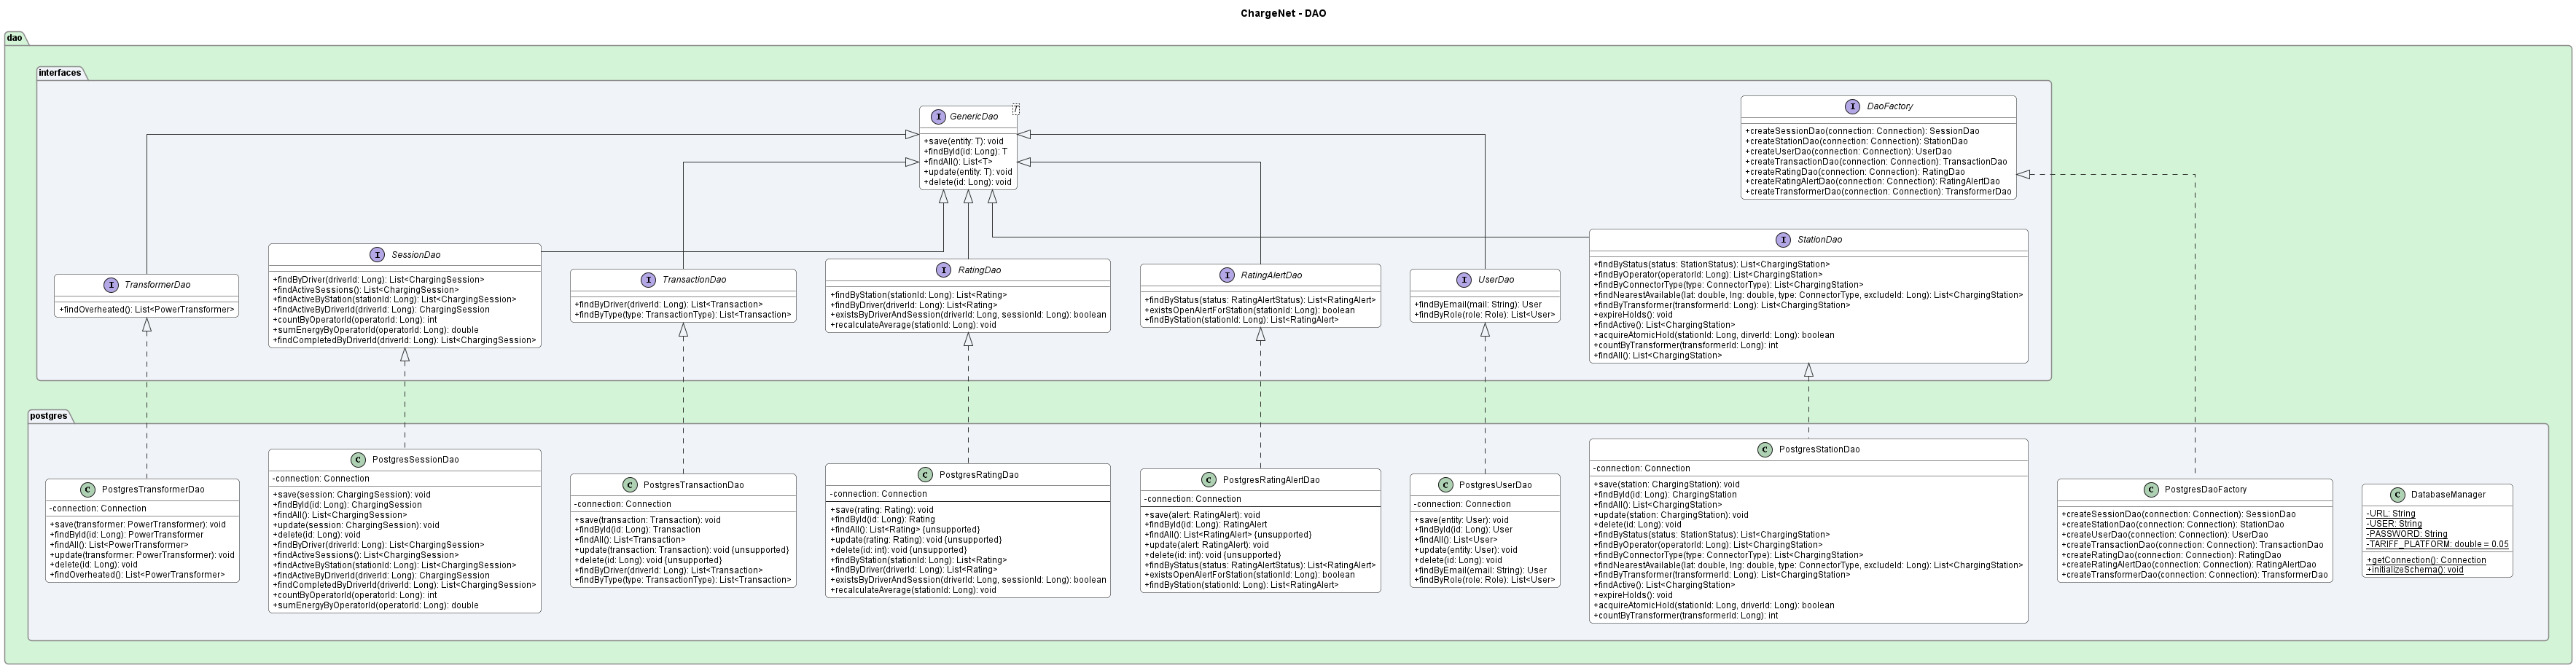
\includegraphics[width=1.10\textwidth]{dao.png}
    \caption{DAO, diagramma di classe}
    \label{fig:DAO}
\end{figure}

\subsection{Presentation Layer}

Il seguente diagramma rappresenta il presentation layer, cioè l'interfaccia grafica dell'applicazione realizzata in JavaFX. Comprende i controller delle varie schermate, che si occupano di mostrare i dati e raccogliere le azioni dell'utente, appoggiandosi ai servizi del livello di business.

\begin{figure}[H]
    \centering
    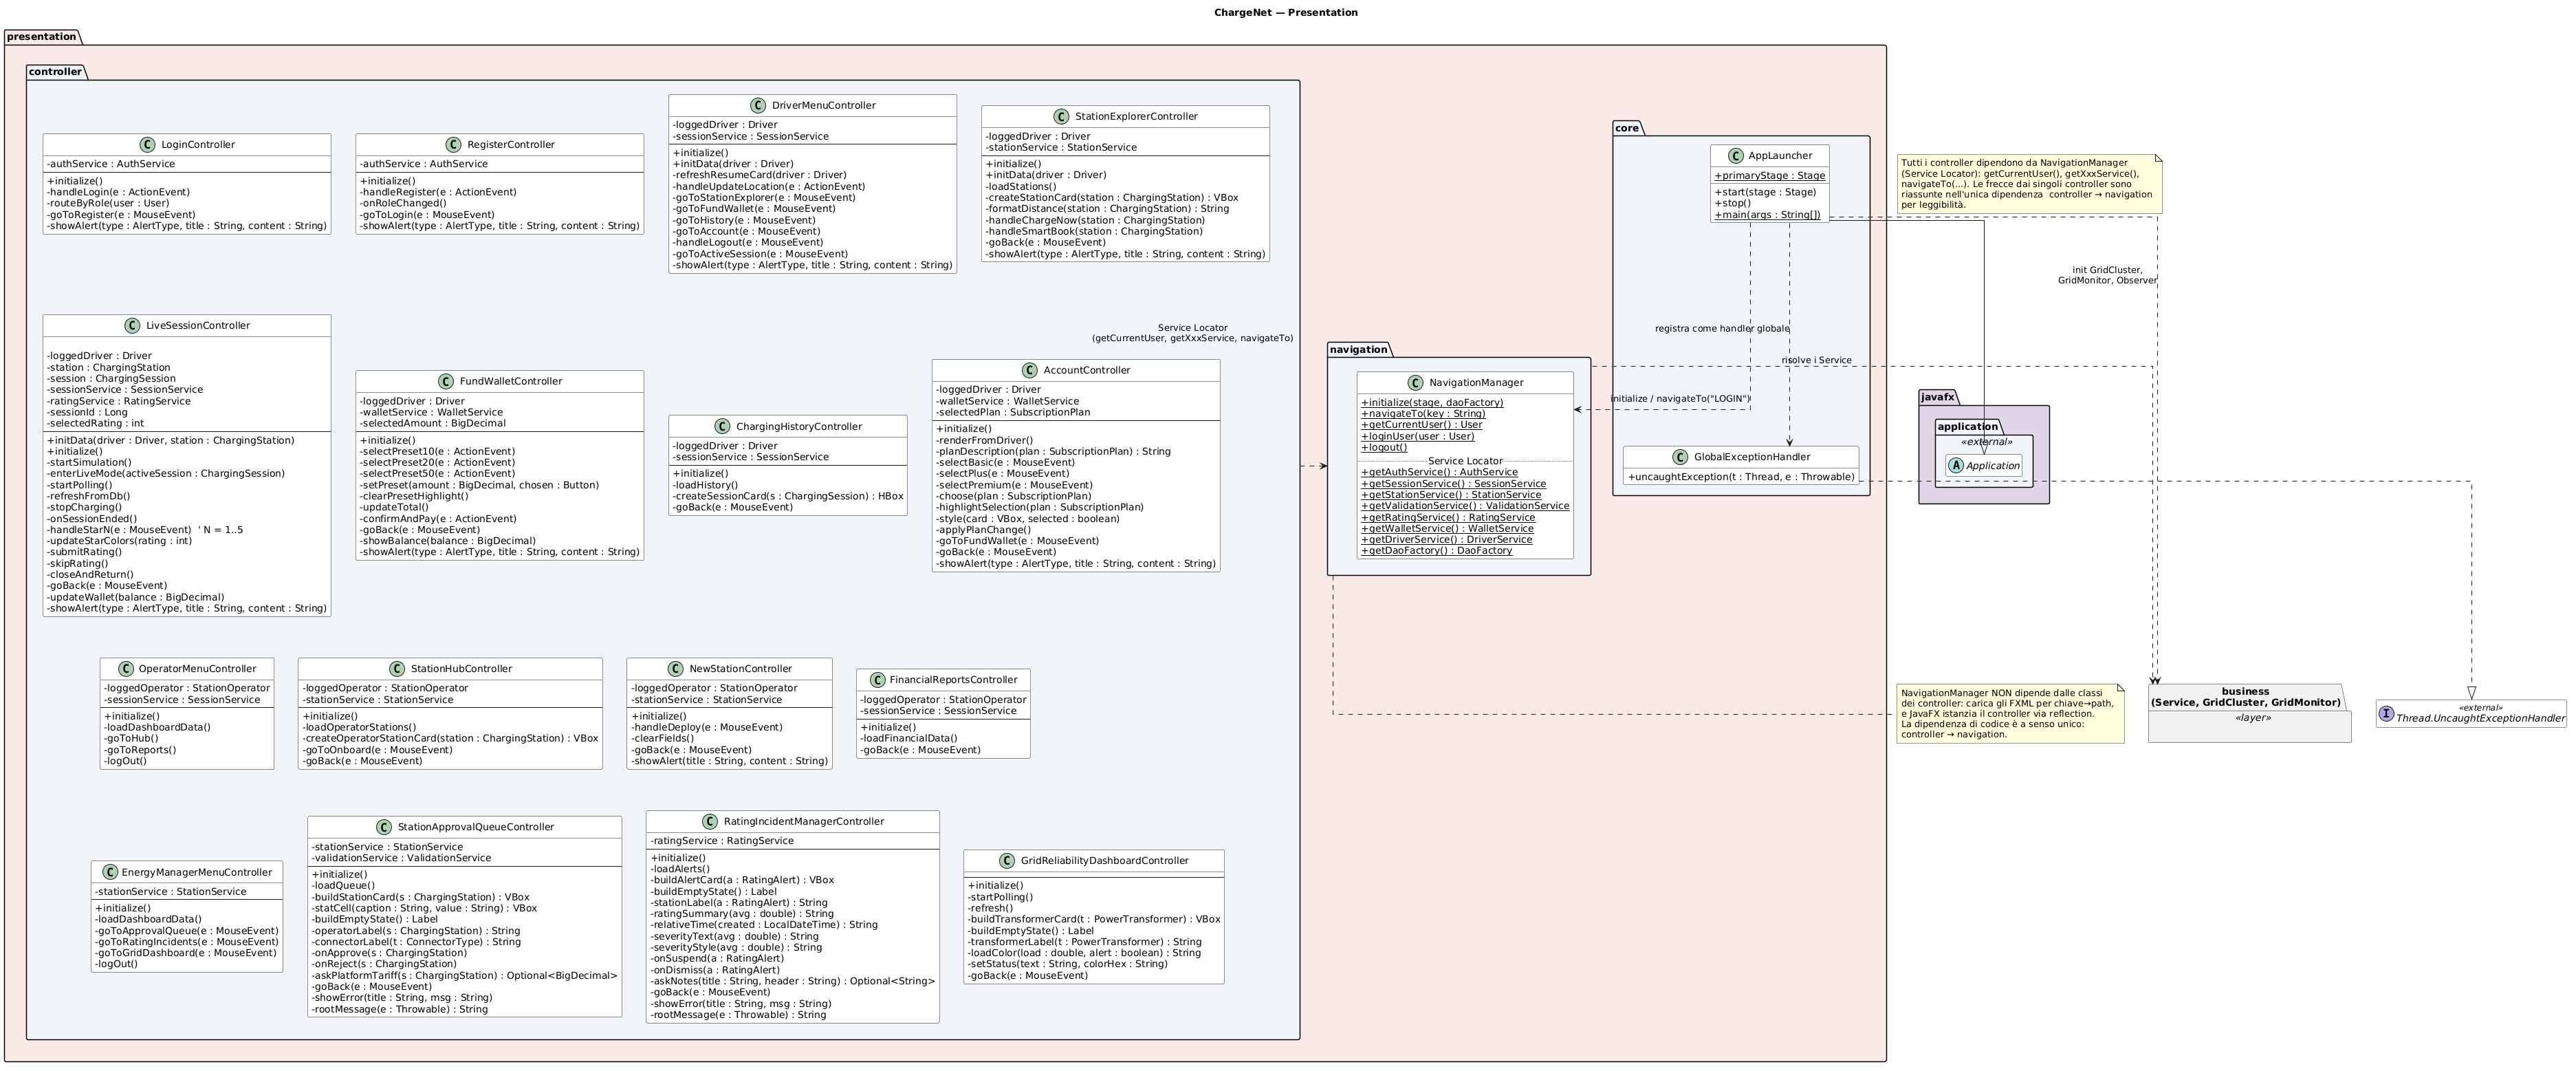
\includegraphics[width=1.10\textwidth]{presentation.png}
    \caption{Presentation Layer, diagramma di classe}
    \label{fig:presentation_layer}
\end{figure}

\section{Sequence Diagram}

Nel seguente paragrafo sono mostrati i diagrammi di sequenza di alcuni dei flussi più significativi del sistema, che descrivono come le varie classi interagiscono tra loro nel tempo per portare a termine un'operazione.

\subsection{Ciclo di vita del GridMonitor
}
\begin{figure}[H]
    \centering
    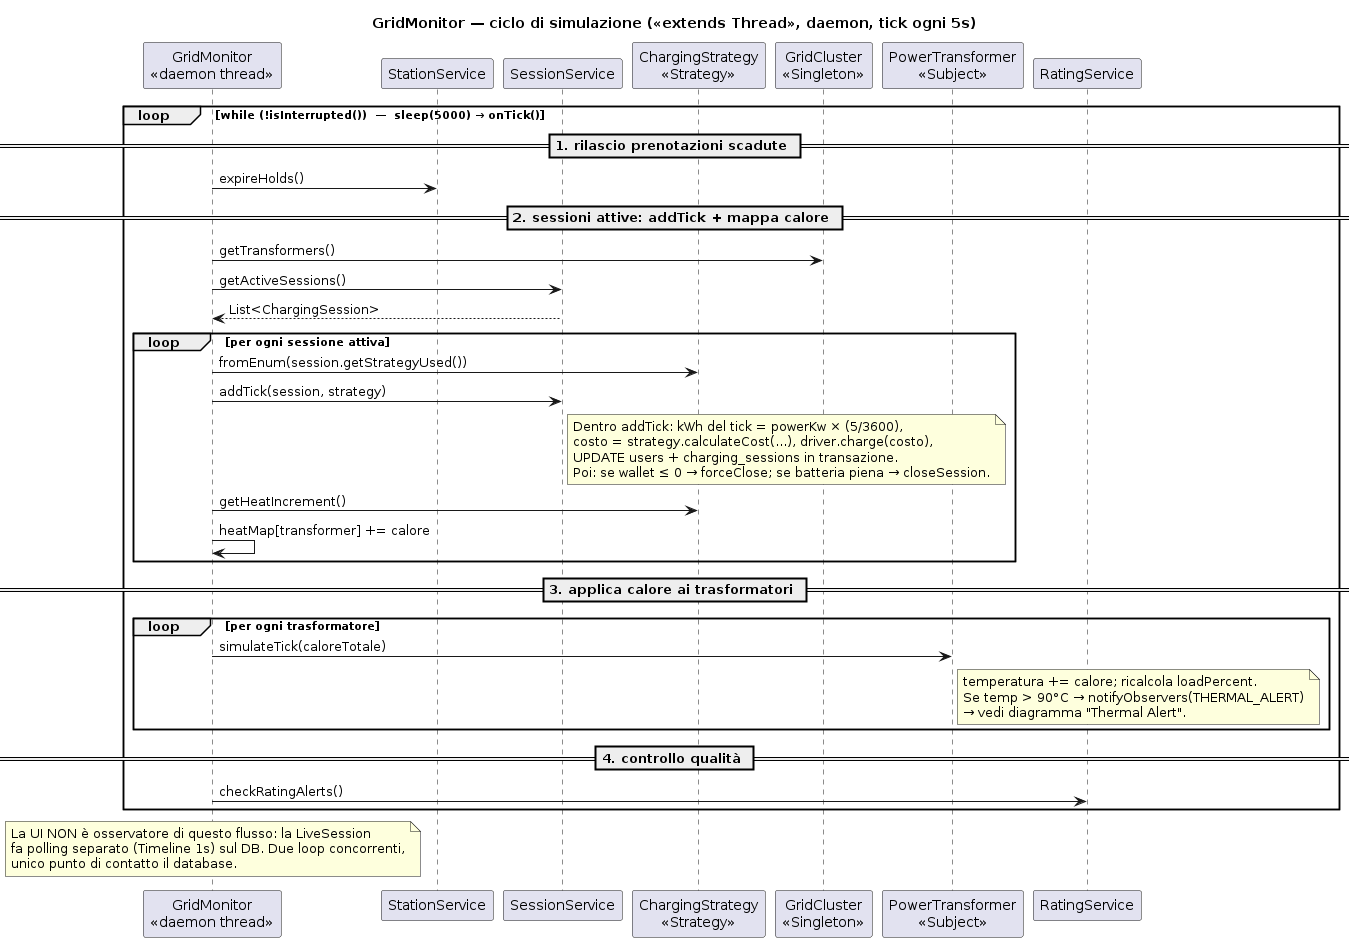
\includegraphics[width=1.10\textwidth]{GridMonitor_Lifecycle.png}
    \caption{Diagramma di sequenza del ciclo di vita del \texttt{GridMonitor}.}
    \label{fig:seq_gridmonitor}
\end{figure}

Il \texttt{GridMonitor} (Fig.~\ref{fig:seq_gridmonitor}) è il thread daemon che scandisce l'intera simulazione della rete elettrica con un tick fisso di 5 secondi, ed è di fatto l'unico componente attivo di propria iniziativa nel sistema: tutti gli altri servizi vengono invocati su richiesta. Ad ogni ciclo il monitor libera prima le prenotazioni scadute tramite \texttt{StationService.expireHolds()}, poi recupera da \texttt{SessionService} l'elenco delle sessioni attive e, per ciascuna, seleziona la \texttt{ChargingStrategy} corrispondente per calcolare kWh erogati e costo del tick, aggiornando in un'unica transazione sia il wallet del Driver sia lo stato della sessione. Lo stesso tick genera un incremento di calore che viene accumulato per trasformatore e applicato a fine ciclo a ciascun \texttt{PowerTransformer}: se la temperatura supera i 90°C viene notificato l'evento \texttt{THERMAL\_ALERT} agli observer registrati, dando origine al flusso descritto in Fig.~\ref{fig:seq_thermal_alert}. Infine il monitor invoca il controllo di qualità del \texttt{RatingService}. È importante osservare che la UI non partecipa a questo ciclo come observer: lo stato delle sessioni viene mostrato tramite un polling separato sul database, in modo tale che i due flussi restino disaccoppiati e l'unico punto di sincronizzazione sia la persistenza.

\subsection{Approvazione di una colonnina}

\begin{figure}[H]
    \centering
    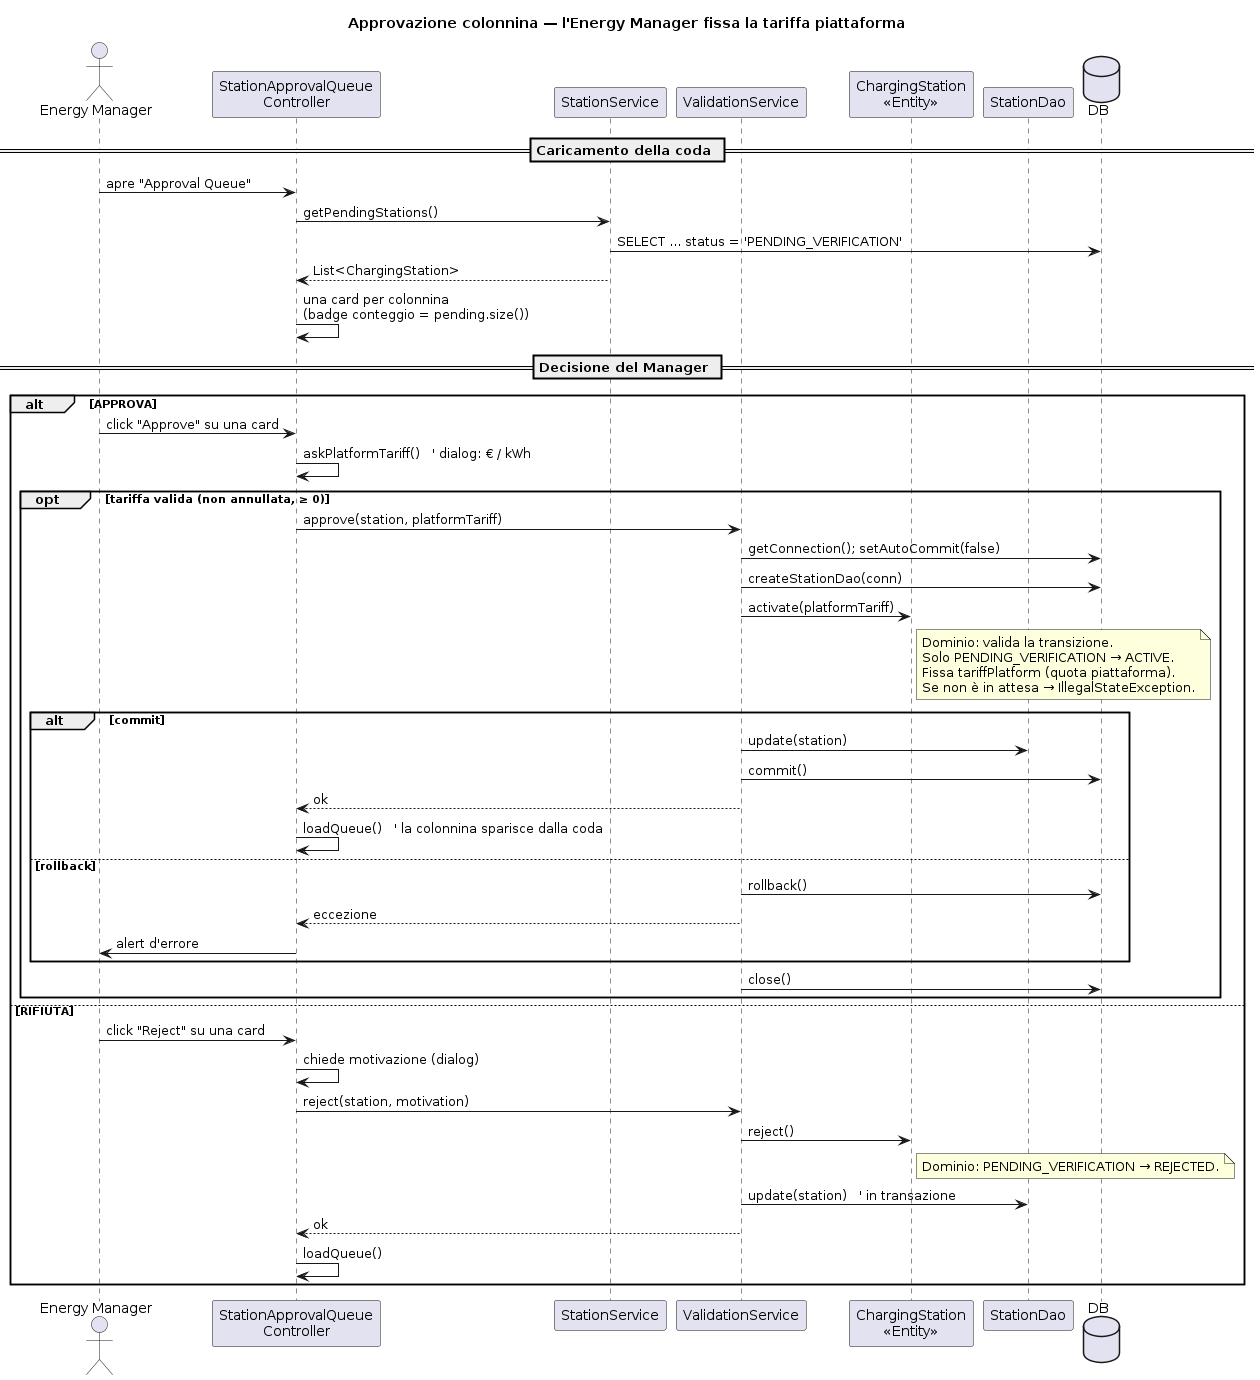
\includegraphics[width=0.9\textwidth]{Station_Approval.png}
    \caption{Diagramma di sequenza dell'approvazione di una colonnina da parte dell'Energy Manager.}
    \label{fig:seq_station_approval}
\end{figure}

Il flusso di approvazione (Fig.~\ref{fig:seq_station_approval}) regola l'ingresso in esercizio di una nuova colonnina proposta da uno Station Operator. L'Energy Manager apre la coda delle richieste in stato \texttt{PENDING\_VERIFICATION}, popolata da \texttt{StationService.getPendingStations()}, e per ciascuna voce può approvare o rifiutare. In caso di approvazione il controller richiede la tariffa di piattaforma da applicare in €/kWh e delega la transizione alla \texttt{ValidationService}, che apre esplicitamente una connessione con \texttt{setAutoCommit(false)} prima di invocare \texttt{activate()} sul dominio: è la \texttt{ChargingStation} stessa a validare che la transizione sia legittima solo a partire da \texttt{PENDING\_VERIFICATION}, sollevando un'eccezione altrimenti, mentre il servizio si occupa unicamente di orchestrare la persistenza e il commit o il rollback della transazione in caso di errore. La stessa separazione si ritrova nel percorso di rifiuto, dove il dominio applica la transizione a \texttt{REJECTED} dopo l'acquisizione della motivazione da parte del Manager. In entrambi i casi la responsabilità di stabilire se un cambio di stato è ammesso resta interamente nel Domain Model , mentre il Business Layer si limita a decidere quando invocarla e a garantirne l'atomicità della persistenza.

\subsection{Gestione dell'evento di temperatura troppo alta (Thermal Alert)}
\begin{figure}[H]
    \centering
    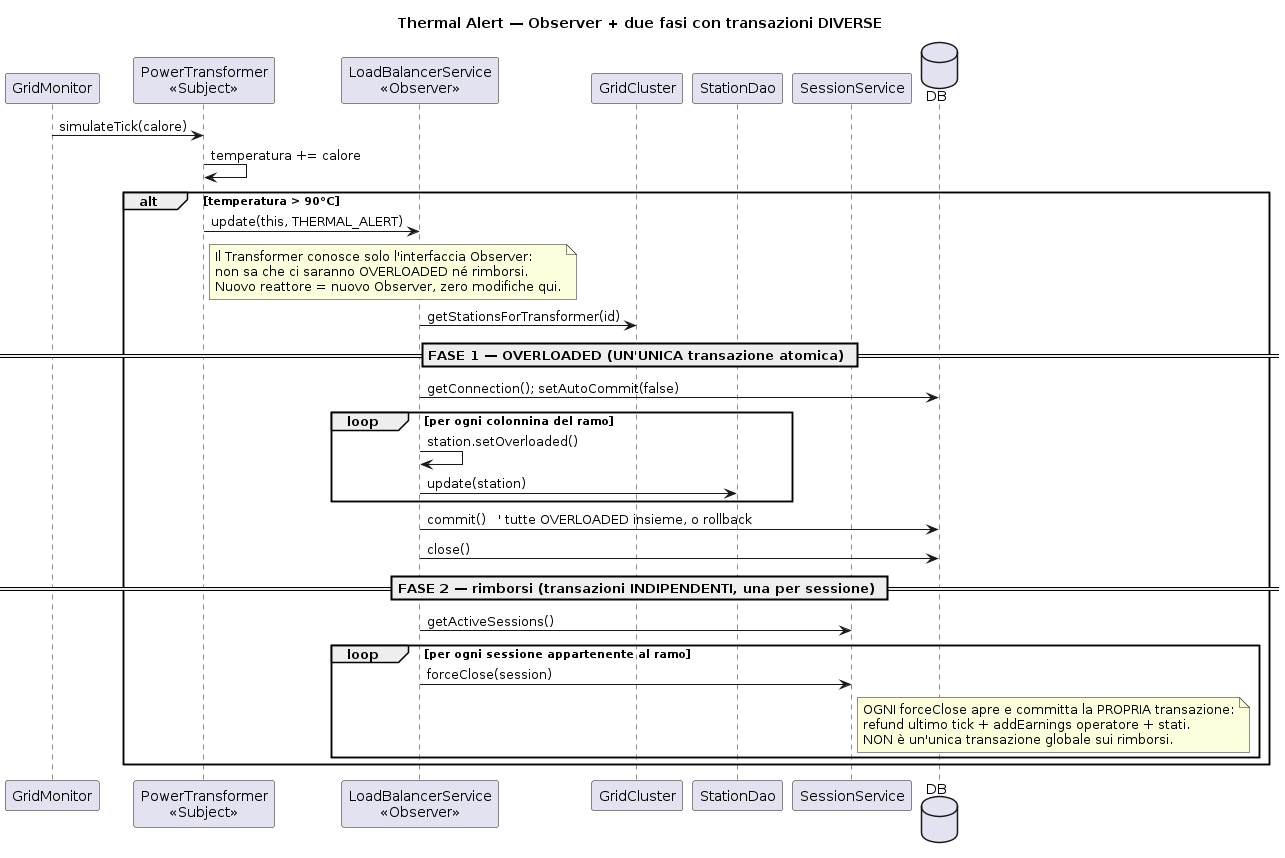
\includegraphics[width=0.9\textwidth]{Thermal_Alert.png}
    \caption{Diagramma di sequenza della gestione di una temperatura troppo alta (Thermal Alert).}
    \label{fig:seq_thermal_alert}
\end{figure}

Il diagramma di Thermal Alert (Fig.~\ref{fig:seq_thermal_alert}) mostra cosa succede quando un trasformatore si surriscalda. Durante il tick del \texttt{GridMonitor}, il \texttt{PowerTransformer} riceve il nuovo carico di calore e aggiorna la propria temperatura interna. Se questa supera i 90°C, il trasformatore avvisa il \texttt{LoadBalancerService}, che è l'unico componente incaricato di reagire all'emergenza: il trasformatore stesso non sa cosa succederà dopo, si limita a segnalare il problema.

A quel punto il \texttt{LoadBalancerService} interviene in due passaggi separati. Nel primo, blocca subito tutte le colonnine collegate a quel trasformatore mettendole in stato \texttt{OVERLOADED}, per evitare che qualcuno continui a ricaricare su un ramo elettrico in sovraccarico: questo blocco viene fatto tutto insieme, colonnina per colonnina, come un'unica operazione che riesce o fallisce nel suo complesso. Nel secondo passaggio, il sistema chiude una per una tutte le sessioni di ricarica che erano attive su quelle colonnine, rimborsando ogni Driver coinvolto tramite \texttt{SessionService.forceClose()}. Qui però ogni chiusura viene trattata singolarmente: se il rimborso di una sessione dovesse fallire, le altre sessioni verrebbero comunque chiuse e rimborsate correttamente, e soprattutto le colonnine resterebbero comunque bloccate in sicurezza, indipendentemente da come va il rimborso.

\section{Database}

La gestione dei dati di ChargeNet è affidata a un database relazionale PostgreSQL. Inizialmente, per velocizzare il lavoro, si è scelto di lavorare inizialmente con H2. Questo ha permesso di scrivere query e testare la parte applicativa fin da subito, per poi occuparsi successivamente dell'installazione e configurazione del database reale, passaggio che è stato comunque rapido visto che non è stato necessario modificare la sintassi SQL (H2 è stato usato in modalità \texttt{MODE=PostgreSQL})

\subsection{Schema ER}

\begin{figure}[H]
    \centering
    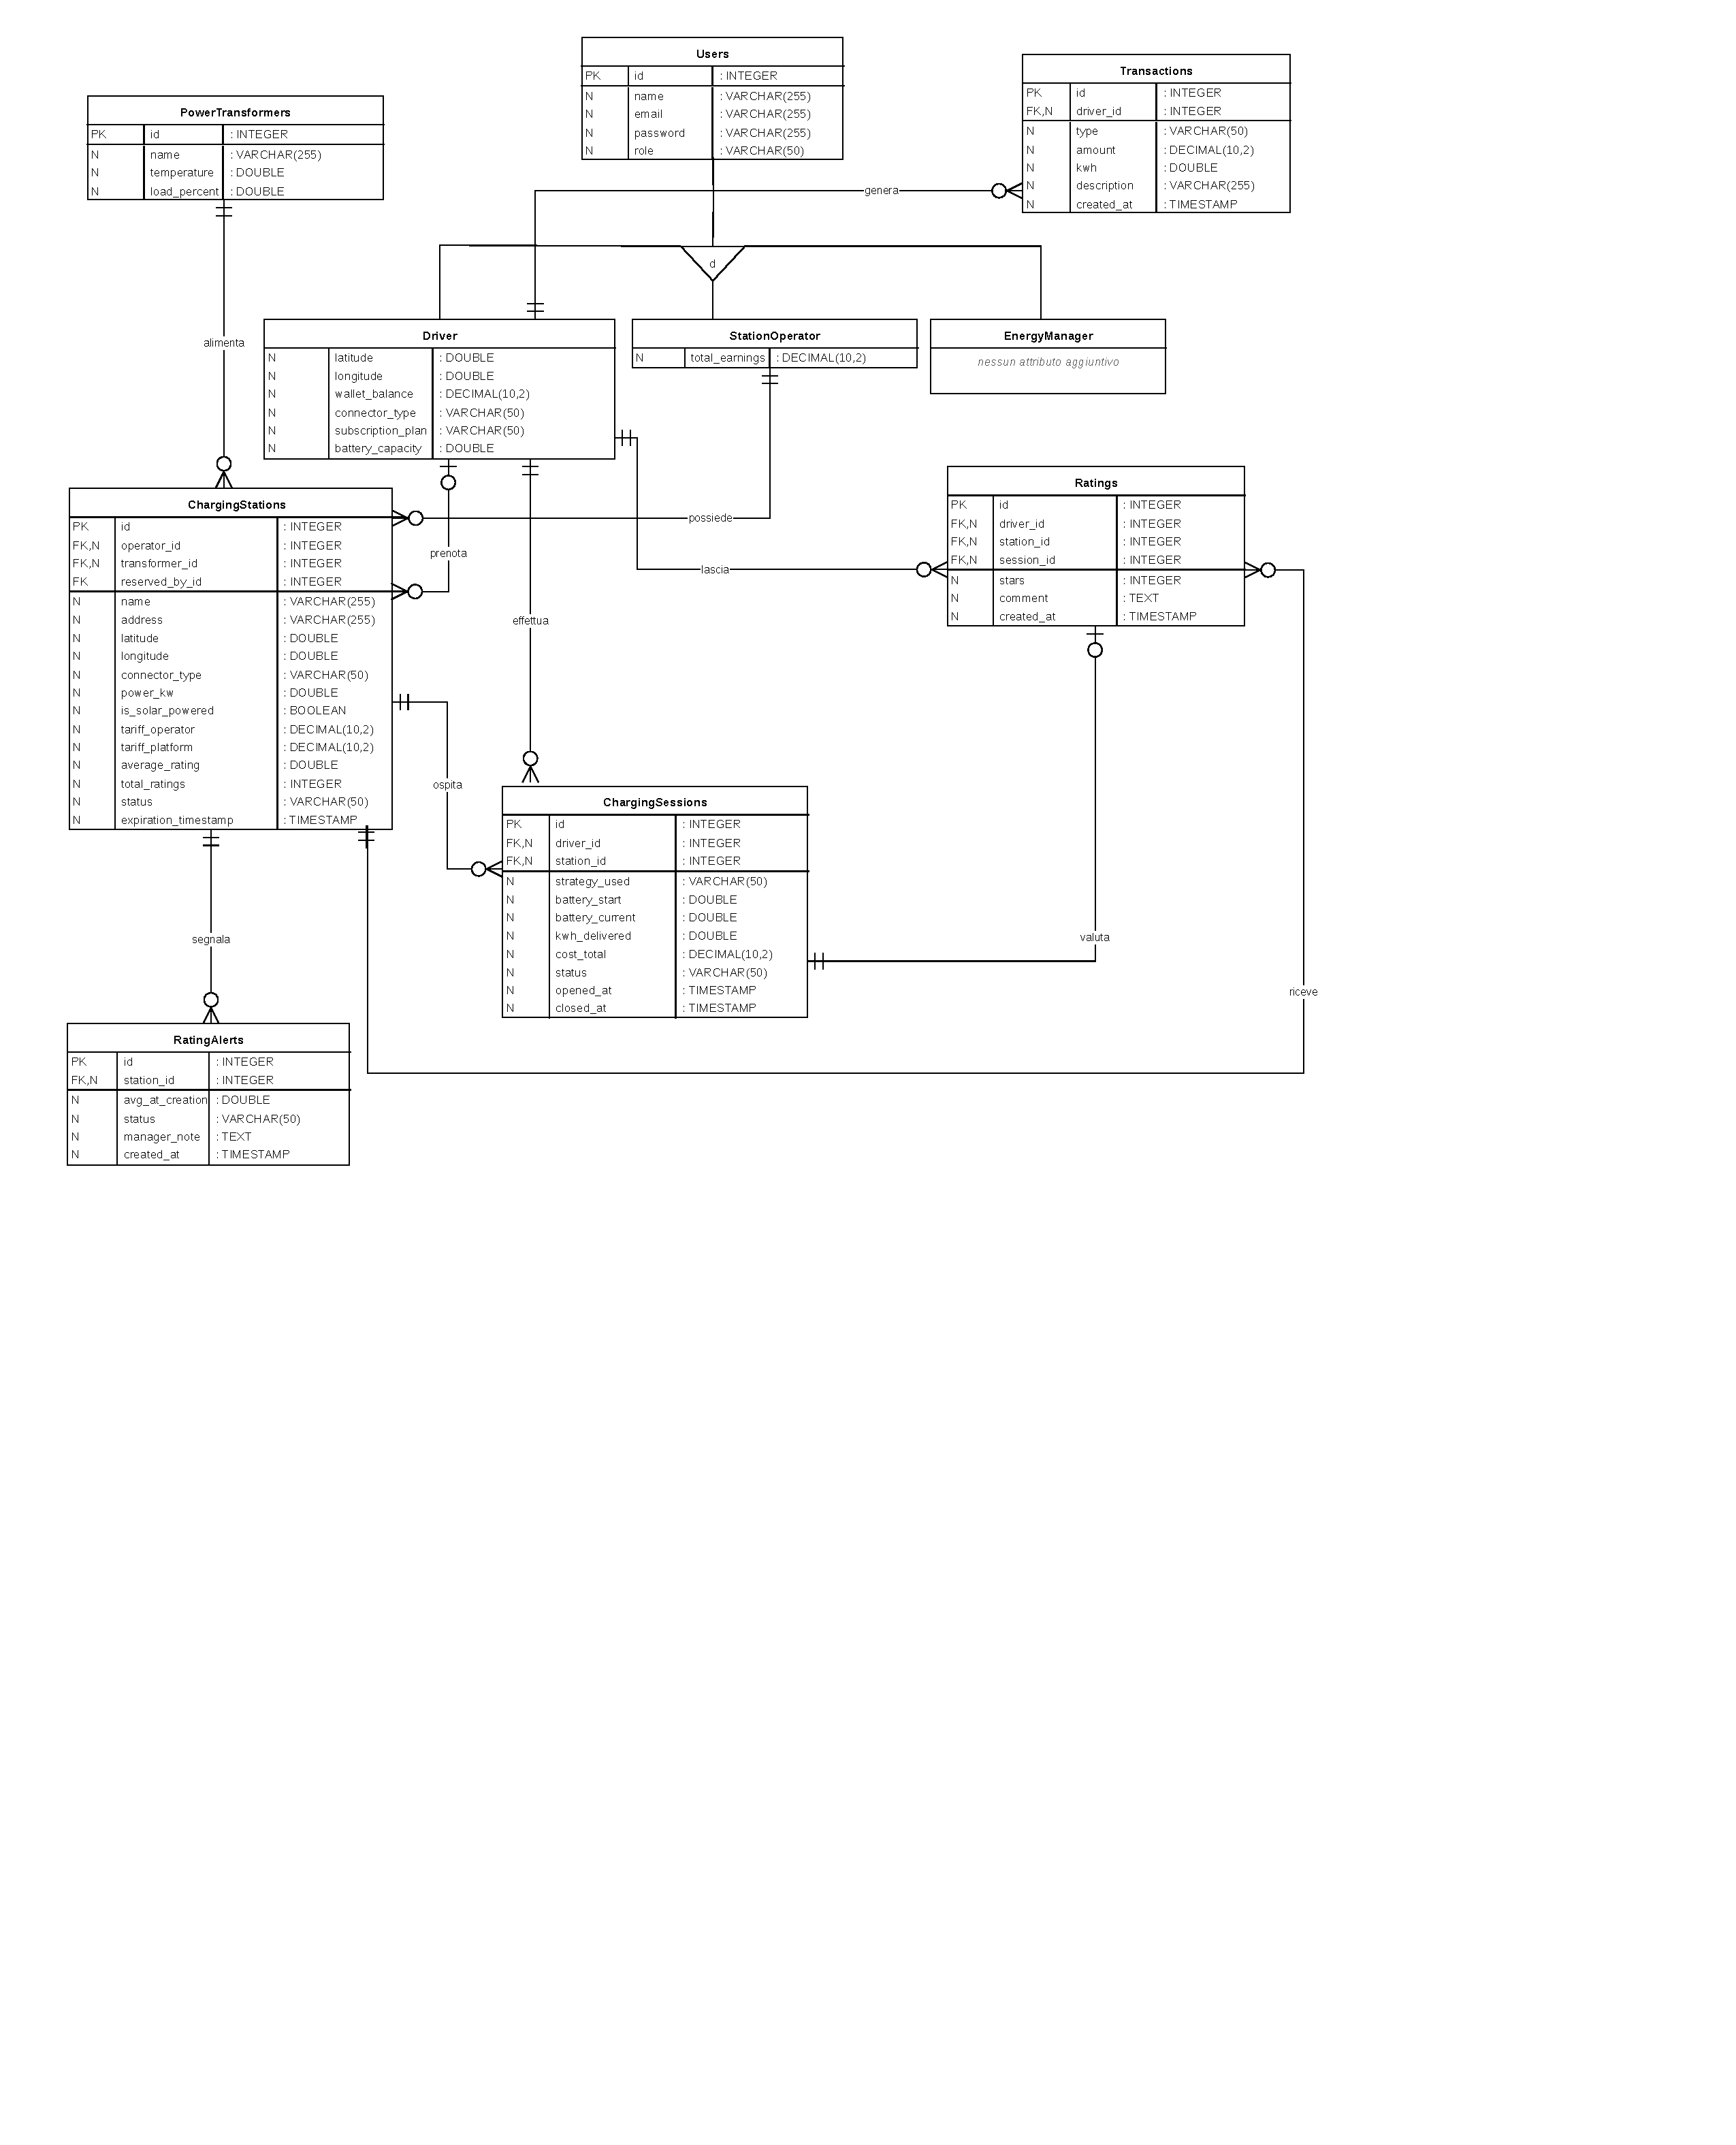
\includegraphics[width=0.95\textwidth]{ChargeNet_ER.drawio.pdf}
    \caption{Schema Entità-Relazione del database ChargeNet.}
    \label{fig:er_chargenet}
\end{figure}

Lo schema (Fig.~\ref{fig:er_chargenet}) riflette la stessa gerarchia già introdotta nel Domain Model: \texttt{Users} è un'entità generica che rappresenta ciò che ogni utente ha in comune (identità, credenziali, ruolo), che viene specializzata in tre sottotipi,\textbf{Driver}, \textbf{StationOperator} ed \textbf{EnergyManager}, ciascuno con i propri attributi specifici. Un utente appartiene esattamente a uno dei tre sottotipi, mai a più di uno contemporaneamente, infatti la colonna \texttt{role} può avere un solo valore.

Le relazioni principali partono dallo specifico sottotipo e non genericamente da \texttt{Users}:

\begin{itemize}
    \item Un \textbf{PowerTransformer} alimenta più \textbf{ChargingStation}.
    \item Uno \textbf{StationOperator} possiede più \textbf{ChargingStation}.
    \item Un \textbf{Driver} può prenotare temporaneamente una colonnina, avviare più \textbf{ChargingSession}, generare più \textbf{Transaction} e lasciare più \textbf{Rating}.
    \item Una \textbf{ChargingStation} ospita più \textbf{ChargingSession} e può ricevere più \textbf{Rating} o generare più \textbf{RatingAlert}.
    \item Ogni sessione può generare al più una \textbf{Rating}.
    \item \textbf{EnergyManager} non compare in nessuna relazione dello schema: il suo ruolo (approvare colonnine, gestire gli alert di qualità) non richiede di possedere o generare entità proprie, ma di agire su entità già esistenti.
\end{itemize}

\subsection{Modello Relazionale}

La traduzione delle entità semplici segue le regole standard: ogni entità diventa una tabella, ogni relazione (1,n) diventa una chiave esterna sul lato "molti". La generalizzazione invece è stata tradotta nel seguente modo: un'unica tabella con tutte le colonne di tutti i sottotipi, dove le colonne che non riguardano una riga restano \texttt{NULL}, e una colonna discriminatore indica il sottotipo reale. 

\begin{quote}
\ttfamily
Users(\uline{id}, name, email, password, role, latitude, longitude, wallet\_balance,\\
\hspace*{3.2em}connector\_type, subscription\_plan, battery\_capacity, total\_earnings)

\vspace{0.8em}
PowerTransformers(\uline{id}, name, temperature, load\_percent)

\vspace{0.8em}
ChargingStations(\uline{id}, \dashuline{operator\_id}, \dashuline{transformer\_id}, name, address,\\
\hspace*{3.2em}latitude, longitude, connector\_type, power\_kw, is\_solar\_powered,\\
\hspace*{3.2em}tariff\_operator, tariff\_platform, average\_rating, total\_ratings,\\
\hspace*{3.2em}status, \dashuline{reserved\_by\_id}$^{\ast}$, expiration\_timestamp)

\vspace{0.8em}
ChargingSessions(\uline{id}, \dashuline{driver\_id}, \dashuline{station\_id}, strategy\_used,\\
\hspace*{3.2em}battery\_start, battery\_current, kwh\_delivered, cost\_total, status,\\
\hspace*{3.2em}opened\_at, closed\_at$^{\ast}$)

\vspace{0.8em}
Transactions(\uline{id}, \dashuline{driver\_id}, type, amount, kwh, description, created\_at)

\vspace{0.8em}
Ratings(\uline{id}, \dashuline{driver\_id}, \dashuline{station\_id}, \dashuline{session\_id}, stars,\\
\hspace*{3.2em}comment, created\_at) \quad \textsc{unique}(driver\_id, session\_id)

\vspace{0.8em}
RatingAlerts(\uline{id}, \dashuline{station\_id}, avg\_at\_creation, status, manager\_note$^{\ast}$, created\_at)
\end{quote}

\vspace{0.3em}
\noindent dove:
\begin{quote}
\ttfamily
operator\_id, reserved\_by\_id \ \ si riferisce a \ \ Users(id)\\
transformer\_id \ \ si riferisce a \ \ PowerTransformers(id)\\
driver\_id \ \ si riferisce a \ \ Users(id)\\
station\_id \ \ si riferisce a \ \ ChargingStations(id)\\
session\_id \ \ si riferisce a \ \ ChargingSessions(id)
\end{quote}

\vspace{1em}
\noindent\textbf{Legenda della notazione}
\begin{itemize}
    \item[] \uline{attributo} \ — \ Chiave Primaria (PK) della tabella.
    \item[] \dashuline{attributo} \ — \ Chiave Esterna (FK) verso un'altra tabella.
    \item[] $^{\ast}$ \ — \ Attributo opzionale (\texttt{NULL} ammesso); tutti gli altri attributi sono obbligatori (\texttt{NOT NULL}).
    \item[] \textsc{unique}(\dots) \ — \ Vincolo di unicità su una combinazione di più colonne.
\end{itemize}

La colonna \texttt{role} in \texttt{Users} dice se la riga rappresenta un Driver, uno StationOperator o un EnergyManager. Colonne come \texttt{wallet\_balance} (Driver) o \texttt{total\_earnings} (StationOperator) esistono per tutte le righe della tabella, ma restano \texttt{NULL} per i sottotipi a cui non appartengono. Per esempio ovviamente non ha senso che \texttt{EnergyManager} abbia un valore diverso da \texttt{null} nell'attributo \texttt{subscription\_plan}. È lo stesso meccanismo già visto nel paragrafo ORM riguardo il metodo \texttt{extractUserFromResultSet()}, che legge la colonna \texttt{role} e ricostruisce l'oggetto Java del sottotipo corretto.


Per quanto riguarda invece le due FK verso \texttt{Users} in \texttt{ChargingStations} (\texttt{operator\_id} e \texttt{reserved\_by\_id}) modellano due relazioni indipendenti — chi possiede la colonnina e chi la sta eventualmente prenotando, ed è proprio per questo che solo la seconda può essere nulla.

Il vincolo \texttt{UNIQUE (driver\_id, session\_id)} sulla tabella \texttt{Ratings} fa si che anche a livello di database valga la regola che un Driver può lasciare una sola valutazione per ciascuna sessione.

Infine, diversi attributi numerici sono protetti da vincoli \texttt{CHECK} direttamente nello schema (es. \texttt{stars} tra 1 e 5, \texttt{wallet\_balance} sempre $\geq 0$): questi vincoli sono una seconda difesa rispetto alla validazione già presente nel Domain Model, indipendente da eventuali bug nel codice Java.

E' presente un limite, conseguenza della generalizzazione utilizzata: la foreign key \texttt{operator\_id} garantisce solo che l'id referenziato esista in \texttt{Users}, non che quella riga appartenga effettivamente a uno StationOperator, lo stesso vale per \texttt{driver\_id} rispetto ai Driver. Questo vincolo di coerenza tra ruolo e utilizzo non è esprimibile a livello di schema relazionale standard, tuttavia è comunque garantito nel codice Java. Infatti il metodo \texttt{StationService.registerStation()} accetta come parametro un \texttt{StationOperator}, non un generico \texttt{User}: un Driver non potrebbe essere passato a quel metodo nemmeno volendo, perché il codice non compilerebbe. La sicurezza che manca allo schema relazionale è quindi comunque garantita ma non appunto da quest'ultimo.
\chapter{Implementazione}

Questo capitolo descrive le scelte implementative e l'architettura interna di ChargeNet. Per mantenere la trattazione chiara, non verrà mostrato l'intero codice sorgente, ma ci si concentrerà sull'organizzazione dei componenti principali e sui frammenti di codice che illustrano le logiche più complesse e i pattern utilizzati. 

\paragraph*{Architettura del Sistema:}

I livelli principali sono tre: Domain, Business e Controller.
L'interazione con il database PostgreSQL è gestita tramite il pattern Data Access Object (DAO), che nasconde la complessità delle query SQL al resto dell'applicazione. 

\section{Domain Model}
 \label{sec: Domain Model}

Per avere maggiore ordine abbiamo suddiviso il Domain Model in cinque pacchetti principali, ognuno con una responsabilità specifica, raggruppando il codice in base alla finalità e al contesto di utilizzo. Questa struttura modulare facilita la manutenzione e l'estensione del sistema, permettendo di isolare le modifiche a specifici ambiti senza impattare l'intero progetto, oltre che a rendere più semplice la comprensione del codice per il lettore.

Di seguito sono elencati i cinque pacchetti principali, con una breve descrizione delle loro responsabilità, che verranno approfondite nel proseguo del paragrafo:
\begin{itemize}
    \item \textbf{Utenti:} Definisce gli attori del sistema. Ci sono tre profili principali (\textit{Driver}, \textit{StationOperator} ed \textit{EnergyManager}), che estendono tutti una classe madre comune per semplificare le operazioni di login e registrazione.
    \item \textbf{Infrastrutture:} Rappresenta le parti fisiche della rete. Contiene le colonnine (\textit{ChargingStation}) e i trasformatori (\textit{PowerTransformer}), e serve a gestire parametri come la potenza massima erogabile o lo stato di occupazione.
    \item \textbf{Sessioni:} È il collegamento pratico tra l'utente e l'infrastruttura. La classe centrale è \textit{ChargingSession}, che si occupa di far partire la ricarica e di calcolare quanti kWh vengono consumati col passare del tempo.
    \item \textbf{Finanze:} Si occupa dei pagamenti e del saldo degli utenti. Gestisce le ricevute (\textit{Transaction}) create dopo una ricarica, un rimborso o il pagamento di un abbonamento, facendo in modo che lo storico contabile non possa essere modificato per sbaglio.
    \item \textbf{Feedback:} Gestisce le recensioni. Raccoglie i voti (\textit{Rating}) lasciati dai guidatori e fa scattare in automatico un avviso di manutenzione (\textit{RatingAlert}) se la media di una stazione si abbassa troppo.
\end{itemize}

Nei prossimi paragrafi vedremo più nel dettaglio alcune delle soluzioni implementative che abbiamo adottato in questi cinque moduli.
\subsection{Utenti}
\label{subsec:utenti}
Questo modulo definisce le identità degli attori tramite un'architettura basata sull'ereditarietà. Dalla classe astratta \texttt{User} derivano i tre profili specifici (\texttt{Driver}, \texttt{StationOperator} ed \texttt{EnergyManager}), ognuno con i propri attributi.

Per rispettare il principio dell'incapsulamento, la logica di business è integrata direttamente nelle entità. Un esempio pratico è la gestione economica del \texttt{Driver}: quando c'è da scalare del credito, è l'oggetto stesso a fare i controlli sul proprio saldo.

\vspace{0,3cm}
\noindent\begin{minipage}{\linewidth}
\begin{lstlisting}[language=Java, caption={Controllo del saldo nel metodo charge()}]
public void charge(BigDecimal amount) {
    if (!hasSufficientBalance(amount)) {
        throw new InsufficientBalanceException("Saldo insufficiente");
    }
    this.walletBalance = this.walletBalance.subtract(amount);
}
\end{lstlisting}
\end{minipage}
\vspace{0.3cm}

Questo approccio torna utile anche per operazioni più delicate. Il cambio di piano, ad esempio, non addebita il canone intero del nuovo piano, ma solo la differenza rispetto a quello attuale, e blocca i downgrade riusando comunque charge() per il controllo del saldo:

\vspace{0,3cm}
\noindent\begin{minipage}{\linewidth}
\begin{lstlisting}[language=Java, caption={Aggiornamento del piano tariffario}]
public BigDecimal updatePlan(SubscriptionPlan newPlan) {
    BigDecimal currentFee = (this.subscriptionPlan != null)
            ? this.subscriptionPlan.getMonthlyFee() : BigDecimal.ZERO;
    BigDecimal delta = newPlan.getMonthlyFee().subtract(currentFee)
            .setScale(2, RoundingMode.HALF_UP);

    if (delta.compareTo(BigDecimal.ZERO) < 0) {
        throw new IllegalArgumentException(
                "Non e possibile passare a un piano inferiore durante il periodo attivo.");
    }
    if (delta.compareTo(BigDecimal.ZERO) > 0) {
        charge(delta);
    }
    this.subscriptionPlan = newPlan;
    return delta;
}
\end{lstlisting}
\end{minipage}
\vspace{0.3cm}

Per il collegamento con il database, invece di passare per i costruttori standard (che farebbero scattare validazioni inutili in fase di caricamento), abbiamo dotato ogni entità di un metodo \texttt{reconstitute()}, pensato esclusivamente per ripristinare in memoria i dati letti da PostgreSQL.

\subsection{Infrastrutture}
L'obiettivo di questo pacchetto è tradurre in codice i limiti fisici del mondo reale. Per la classe \texttt{ChargingStation} era fondamentale impedire la creazione di oggetti con parametri incoerenti o pericolosi.

Abbiamo quindi nascosto i costruttori, obbligando il resto del sistema a passare per il Factory Method \texttt{register()}. In questa fase la stazione esegue quattro controlli in sequenza: coordinate geografiche valide, potenza compresa tra 7 e 350 kW, potenza compatibile col limite fisico del connettore, e tariffa dell'operatore positiva. Basta che uno fallisca per bloccare subito la creazione.

\vspace{0.3cm}
\noindent\begin{minipage}{\linewidth}
\begin{lstlisting}[language=Java, caption={Factory Method per la registrazione della stazione}]
public static ChargingStation register(StationOperator operator, PowerTransformer transformer,
                                        String name, String address, Double lat, Double lng,
                                        ConnectorType connectorType, Double powerKw,
                                        Boolean isSolar, BigDecimal tariff) {
    if (lat < -90.0 || lat > 90.0) {
        throw new InvalidStationParametersException("Latitudine non valida");
    }
    if (lng < -180.0 || lng > 180.0) {
        throw new InvalidStationParametersException("Longitudine non valida");
    }
    if (powerKw < 7.0 || powerKw > 350.0) {
        throw new InvalidStationParametersException("Potenza non valida. Deve essere compresa tra 7 kW e 350 kW.");
    }
    if (powerKw > connectorType.getMaxPowerKw()) {
        throw new InvalidStationParametersException("Errore di sicurezza: La potenza richiesta (" + powerKw +
                " kW) supera il limite fisico supportato dal connettore " + connectorType.name() +
                " (" + connectorType.getMaxPowerKw() + " kW).");
    }
    if (tariff.compareTo(BigDecimal.ZERO) <= 0) {
        throw new InvalidStationParametersException("La tariffa dell'operatore deve essere strettamente positiva.");
    }
    return new ChargingStation(operator, transformer, name, address, lat, lng, connectorType, powerKw, isSolar, tariff);
}
\end{lstlisting}
\end{minipage}
\vspace{0.3cm}

L'altro parte fodnamentale del pacchetto è il \texttt{PowerTransformer}, che fa da base per il sistema di Load Balancing. Piuttosto che avere un servizio esterno che controlla continuamente i trasformatori, abbiamo reso il trasformatore intelligente applicando il pattern Observer. A ogni ciclo di simulazione, ricalcola la sua temperatura interna; se supera la soglia critica dei 90 gradi, genera autonomamente un \texttt{THERMAL\_ALERT} per avvisare la rete, senza bisogno di sapere chi o come gestirà effettivamente l'emergenza(vedasi paragrafo~\ref{sec: Observer Pattern}).

\subsection{Sessioni}
Il pacchetto racchiude la logica legata all'erogazione dell'energia. La classe centrale, \texttt{ChargingSession}, non si limita a registrare passivamente i dati (come kWh erogati e costi parziali), ma regola attivamente l'intero ciclo di vita dell'operazione, dalla creazione fino al completamento naturale o all'interruzione per emergenza termica.

Per garantire che una ricarica non inizi in condizioni non valide, l'istanziazione è affidata al metodo factory \texttt{open()}. Questo metodo esegue una serie di controlli incrociati di dominio: verifica la compatibilità fisica del connettore, controlla che la stazione non sia occupata e delega a ChargingStation.priceFor() il calcolo del saldo minimo richiesto, lo stesso metodo che userà poi la strategia di ricarica scelta, così il controllo d'ingresso e l'addebito reale non possono mai calcolare cifre diverse:

\vspace{0.3cm}
\noindent\begin{minipage}{\linewidth}
\begin{lstlisting}[language=Java, caption={Apertura di una sessione di ricarica}]
public static ChargingSession open(Driver driver, ChargingStation station, ChargingType strategy, Double batteryStart) {

    boolean isAvailable = station.isAvailableFor(driver.getConnectorType()) || station.isReservedBy(driver);
    if (!isAvailable) {
        throw new StationNotAvailableException("La colonnina " + station.getName() + " non e' disponibile o non e' compatibile col tuo veicolo.");
    }

    BigDecimal minimumRequired = station.priceFor(5.0, driver);

    if (!driver.hasSufficientBalance(minimumRequired)) {
        throw new InsufficientBalanceException("Credito insufficiente per avviare la sessione. E' richiesto un saldo di almeno " +
                minimumRequired + "\\texteuro.");
    }

    return new ChargingSession(driver, station, strategy, batteryStart);
}
\end{lstlisting}
\end{minipage}
\vspace{0.5cm}

Inoltre, la classe incapsula la logica di avanzamento tramite il metodo \texttt{addTick()}, che aggiorna in tempo reale i costi e l'energia immessa, facendo transitare automaticamente lo stato della sessione a completato qualora la batteria raggiunga il 100\% della sua capacità.

\subsection{Finanze}
Questo modulo gestisce lo storico dei movimenti economici degli utenti, categorizzandoli tramite l'enumerazione \texttt{TransactionType} (ricariche, rimborsi, abbonamenti e depositi). 

La scelta architetturale più rilevante per l'entità \texttt{Transaction} è stata quella di renderla intrinsecamente immutabile. Trattandosi di dati contabili, era fondamentale garantire che uno storico non potesse essere alterato accidentalmente a runtime. Per questo motivo, la classe è sprovvista di metodi \textit{setter} e i suoi campi sono valorizzabili unicamente al momento della creazione.

Per blindare ulteriormente l'integrità del registro, la generazione di un nuovo movimento non avviene tramite un normale costruttore, ma è protetta da un metodo factory che scarta a priori qualsiasi operazione anomala, come ad esempio i pagamenti a importo zero o privi di causale:

\vspace{0.3cm}
\noindent\begin{minipage}{\linewidth}
\begin{lstlisting}[language=Java, caption={Creazione di una transazione contabile}]
public static Transaction create(Driver driver, TransactionType type, BigDecimal amount,
                                 Double kwh, String description) {

    if (amount == null || amount.compareTo(BigDecimal.ZERO) == 0) {
        throw new IllegalArgumentException("Errore: l'importo non puo' essere zero.");
    }
    if (description == null || description.trim().isEmpty()) {
        throw new IllegalArgumentException("Errore: la transazione deve avere una descrizione.");
    }
    return new Transaction(driver, type, amount, kwh, description);
}
\end{lstlisting}
\end{minipage}
\vspace{0.3cm}

Questa impostazione si è rivelata molto utile per semplificare la logica del livello Business, sapendo di poter fare affidamento su un tracciamento finanziario solido e privo di "transazioni fantasma".

\subsection{Feedback}
A chiudere il Domain Model troviamo la parte dedicata alla qualità del servizio e al supporto. Qui abbiamo deciso di separare l'azione dell'utente (la recensione) dalla conseguente gestione amministrativa (l'allarme per la manutenzione).

Nella classe \texttt{Rating}, la creazione di un nuovo feedback è protetta da controlli rigorosi. Abbiamo implementato il metodo factory \texttt{leave()}, che non si limita a istanziare la recensione, ma lega quest'ultima alla sessione di ricarica effettiva e impedisce l'inserimento di voti fuori dal range previsto:

\vspace{0.3cm}
\noindent\begin{minipage}{\linewidth}
\begin{lstlisting}[language=Java, caption={Creazione di un feedback utente}]
public static Rating leave(Driver driver, ChargingStation station, ChargingSession session, Integer stars, String comment) {
    if (stars == null || stars < 1 || stars > 5) {
        throw new InvalidRatingException("Errore di validazione: il rating deve essere un valore compreso tra 1 e 5 stelle.");
    }
    return new Rating(driver, station, session, stars, comment);
}
\end{lstlisting}
\end{minipage}
\vspace{0.3cm}

Una parte interessante di questo modulo si trova nella classe \texttt{RatingAlert}. Quando la media di una stazione cala drasticamente, il sistema genera un avviso. Invece di affidare la chiusura di questo ticket a un servizio esterno, abbiamo inserito la logica di transizione di stato direttamente all'interno dell'entità. I metodi per sospendere la colonnina o ignorare l'allarme verificano prima che la segnalazione sia effettivamente ancora in sospeso, evitando che un operatore possa inavvertitamente alterare pratiche già chiuse, La decisione di generare l'alert, invece, non spetta al dominio ma al RatingService (vedi paragrafo \ref{sec:GestioneFeedback}), che dopo ogni nuova recensione ricalcola la media e verifica la soglia.

\vspace{0.3cm}
\noindent\begin{minipage}{\linewidth}
\begin{lstlisting}[language=Java, caption={Chiusura di un alert di manutenzione}]
public void resolveSuspend(String note) {
    if (isPending()) {
        this.status = RatingAlertStatus.RESOLVED_SUSPENDED;
        this.managerNote = note;
    }
}
\end{lstlisting}
\end{minipage}

\section{Business Layer}
\label{sec: Business}
Il Business Layer rappresenta il livello in cui i dati del Domain Model vengono elaborati e trasformati in funzionalità concrete. L'architettura di questo strato è stata progettata seguendo il principio di singola responsabilità (SRP), suddividendo il codice in servizi specializzati (\textit{Services}) e componenti di simulazione (\textit{Core}).

L'implementazione delle diverse logiche di erogazione (\textit{ChargingStrategy}) verrà approfondita nella successiva sezione dedicata ai Design Pattern.

Di seguito vengono analizzate nel dettaglio le classi centrali che governano e dirigono il flusso dell'applicazione.

\subsection{GridCluster}
Il primo problema tecnico che abbiamo affrontato progettando la simulazione è stato il carico sul database. Poiché il sistema deve ricalcolare i consumi e le temperature della rete ogni pochi secondi, eseguire continuamente query di lettura tramite i DAO avrebbe rallentato l'intera applicazione.

Per risolvere questo collo di bottiglia, abbiamo implementato \texttt{GridCluster}. Si tratta di una cache in memoria, gestita come Singleton, che viene popolata una sola volta all'avvio dell'applicazione. Al suo interno, i dati non sono salvati in semplici liste, ma indicizzati strategicamente tramite mappe Hash per garantire tempi di accesso costanti ($O(1)$). Ad esempio, raggruppando le colonnine per ID del trasformatore, il sistema può recuperare l'intero ramo di rete istantaneamente:

\vspace{0.3cm}
\noindent\begin{minipage}{\linewidth}
\begin{lstlisting}[language=Java]

private Map<Long, List<ChargingStation>> stationsByTransformer;

 public void init(TransformerDao tDao, StationDao sDao) {
        this.transformers = tDao.findAll();
        this.allStations = sDao.findAll();

        for (PowerTransformer t : transformers) {
            stationsByTransformer.put(t.getId(), new ArrayList<>());
        }

        for (ChargingStation station : allStations) {
            Long tId = station.getTransformer().getId();
            if (stationsByTransformer.containsKey(tId)) {
                stationsByTransformer.get(tId).add(station);
            }
        }
    }

\end{lstlisting}
\end{minipage}
\vspace{0.3cm}

Oltre alla gestione della rete elettrica, questa classe espone anche i metodi di ricerca geografica, utilizzando la distanza euclidea per restituire rapidamente all'utente le colonnine disponibili più vicine.

\subsection{GridMonitor}
 Non avendo a disposizione dei sensori fisici che inviano dati telemetrici, avevamo bisogno di un componente che facesse scorrere il tempo in modo autonomo, senza bloccare l'interfaccia grafica.

Abbiamo quindi esteso la classe \texttt{Thread} di Java. Un dettaglio implementativo fondamentale è stato impostare questo thread come "Demone" all'interno del costruttore (\texttt{this.setDaemon(true);}). In questo modo, il ciclo vitale del monitor viene legato a quello dell'interfaccia JavaFX: se l'utente chiude la finestra dell'applicazione, il thread si arresta in modo pulito senza lasciare processi appesi in background.

Il ciclo di esecuzione principale si sveglia ogni 5 secondi e orchestra le operazioni dei vari servizi, aggregando i dati prima di applicarli:

\vspace{0.2cm}
\noindent\begin{minipage}{\linewidth}
\begin{lstlisting}[language=Java]
private void onTick() {
    
    expireShortTermHolds();

    Map<PowerTransformer, Double> heatMap = processActiveSessions();

    processTransformers(heatMap);

    checkRatingAlerts();
}
\end{lstlisting}
\end{minipage}
\vspace{0.3cm}

In particolare, la fase di elaborazione (\texttt{processActiveSessions}) calcola il calore generato dalle singole strategie di ricarica in uso (Fast o Eco) e lo somma all'interno di una \textit{Heat Map}, in modo da notificare i trasformatori una sola volta per ciclo, ottimizzando ulteriormente le prestazioni.

\subsection{LoadBalancerService}
Il \texttt{LoadBalancerService} è il componente che giustifica l'esistenza del pattern Observer all'interno dell'architettura. Invece di interrogare attivamente la rete per scovare eventuali surriscaldamenti, questo servizio si registra semplicemente in ascolto sui trasformatori. 

Quando riceve una notifica di \texttt{THERMAL\_ALERT}, il servizio reagisce isolando immediatamente il ramo di rete compromesso. L'intervento si divide in due fasi distinte, con garanzie transazionali deliberatamente diverse. Nella \textbf{prima fase} viene aperta un'unica transazione che porta a \texttt{OVERLOADED} tutte le colonnine collegate al trasformatore, impedendo l'avvio di nuove ricariche: o passano tutte, o non ne passa nessuna. Questa transazione viene poi \emph{chiusa prima} di passare alla seconda fase, e non per un problema di deadlock, ma per una ragione più semplice: la \textbf{seconda fase} delega la chiusura delle sessioni in corso al \texttt{SessionService}, che apre connessioni proprie: tenere aperta la connessione della prima fase mentre se ne aprono altre sulle stesse righe significherebbe contendere inutilmente i lock che quella transazione ha già acquisito. Chiuderla per tempo li rilascia.

\vspace{0.3cm}
\noindent\begin{minipage}{\linewidth}
\begin{lstlisting}[language=Java, caption={Gestione dell'alert termico}]
private void handleThermalAlert(PowerTransformer transformer) {
    
    Connection connection = null;
    try {
        connection = DatabaseManager.getConnection();;
        connection.setAutoCommit(false);
        StationDao stationDao = daoFactory.createStationDao(connection);

        for (ChargingStation station : stations) {
            station.setOverloaded();
            stationDao.update(station);
        }
        connection.commit();
    } finally {
        closeQuietly(connection); // Previene blocchi a cascata
    }

    
    for (ChargingSession session : sessionService.getActiveSessions()) {
        if (belongsToTransformer(session.getStation(), stations)) {
            sessionService.forceClose(session);
        }
    }
}
\end{lstlisting}
\end{minipage}
\vspace{0.3cm}

È importante notare che questa seconda fase non è atomica nel suo complesso: ogni chiusura forzata (\texttt{forceClose}) apre e chiude una propria transazione indipendente, invece di essere racchiusa in un'unica transazione che copra tutte le sessioni del ramo. È una scelta deliberata, non un limite del sistema: se il fallimento di un singolo rimborso facesse fallire anche gli altri già conclusi con successo, si penalizzerebbero driver che non hanno responsabilità in quel fallimento.

Ogni chiusura forzata produce due effetti economici distinti, salvati nella stessa transazione, il rimborso al Driver e l'accredito
allo Station Operator.

\vspace{0.3cm}
\noindent\begin{minipage}{\linewidth}
\begin{lstlisting}[language=Java, caption={Rimborso e accredito in forceClose()}]
double kwhLastTick = station.getPowerKw() * (5.0 / 3600.0);
BigDecimal refundAmount = BigDecimal.valueOf(
    strategy.calculateCost(kwhLastTick, station, session.getDriver()));

if (wasActive && station.getOperator() != null) {
    double kwhDelivered = session.getKwhDelivered();
    BigDecimal operatorShare = station.getTariffOperator()
        .multiply(BigDecimal.valueOf(kwhDelivered))
        .setScale(2, RoundingMode.HALF_UP);
    operator.addEarnings(operatorShare);
    userDao.update(operator);
}
\end{lstlisting}
\end{minipage}
\vspace{0.3cm}

Il Driver viene rimborsato solo del costo dell'ultimo tick da 5 secondi, cioè
l'energia pagata ma non ancora erogata al momento dello stacco. Lo Station
Operator, allo stesso tempo, viene comunque accreditato della propria quota
sull'intera energia realmente erogata fino a quel punto. L'interruzione non annulla quindi l'intera operazione: divide il conto tra le due parti in base a cosa è realmente accaduto prima dello stop.

\subsubsection*{Il ritorno in servizio: l'isteresi termica}

L'emergenza però non è uno stato definitivo, e il \texttt{LoadBalancerService} gestisce anche la strada del ritorno. Il trasformatore non ha una soglia sola, ma \textbf{due}: una di \emph{allarme} a 90\,°C, oltre la quale scatta il \texttt{THERMAL\_ALERT} appena descritto, e una di \emph{rientro} più bassa, a 70\,°C. Quando la temperatura, non essendoci più ricariche attive su quel ramo, ridiscende sotto i 70\,°C, il trasformatore emette un secondo evento, \texttt{COOLING\_COMPLETE}, che lo stesso observer intercetta per riportare ad \texttt{ACTIVE} tutte e sole le colonnine rimaste in \texttt{OVERLOADED}, di nuovo in un'unica transazione.

\vspace{0.3cm}
\noindent\begin{minipage}{\linewidth}
\begin{lstlisting}[language=Java, caption={Rientro in servizio dopo il raffreddamento}]
private void handleCoolingComplete(PowerTransformer transformer) {
    List<ChargingStation> stations =
        GridCluster.getInstance().getStationsForTransformer(transformer.getId());
    ...
    for (ChargingStation station : stations) {
        if (station.getStatus() == StationStatus.OVERLOADED) {
            station.setActive();
            stationDao.update(station);
        }
    }
    connection.commit();
    ...
}
\end{lstlisting}
\end{minipage}
\vspace{0.3cm}

La distanza tra le due soglie non è arbitraria: è un'\textbf{isteresi}, ed è ciò che impedisce al sistema di oscillare. Con una soglia sola, un trasformatore fermo esattamente sul valore critico riattiverebbe le colonnine, che ricomincerebbero subito a scaldare, facendolo risalire sopra la soglia e provocando un nuovo blocco: un ciclo di accensioni e spegnimenti a raffica. Imponendo che per rientrare si debba scendere \emph{ben sotto} il punto in cui si è usciti, il sistema si concede un margine di raffreddamento reale prima di riaprire il ramo. È lo stesso principio del termostato di casa, che non riaccende la caldaia al primo decimo di grado sotto la temperatura impostata. Il filtro \texttt{if (station.getStatus() == OVERLOADED)} garantisce inoltre che il rientro riguardi solo le colonnine spente dall'emergenza, senza risvegliare quelle che si trovano in altri stati per ragioni indipendenti (per esempio sospese dall'Energy Manager per qualità scadente).

\subsection{SessionService}
\label{subsec:sessionservice}
Mentre il \texttt{LoadBalancerService} gestisce le emergenze, il \texttt{SessionService} governa la normale operatività economica ed energetica: è il servizio più sollecitato del sistema, invocato ad ogni tick del \texttt{GridMonitor} per ciascuna sessione in corso.

\subsubsection*{Il denaro si scala tick per tick, non a fine ricarica}

È il punto che più spesso viene frainteso, ed è bene fissarlo subito: \textbf{il portafoglio del Driver non viene addebitato al termine della ricarica, ma progressivamente, cinque secondi alla volta, dal motore di simulazione.} Ogni tick calcola l'energia erogata nell'intervallo (la potenza della colonnina moltiplicata per la frazione d'ora corrispondente), ne chiede il costo alla \texttt{ChargingStrategy} in uso, e scala subito quella cifra dal saldo:

\vspace{0.3cm}
\noindent\begin{minipage}{\linewidth}
\begin{lstlisting}[language=Java, caption={Avanzamento di una ricarica: addebito e persistenza in un'unica transazione}]
public void addTick(ChargingSession session, ChargingStrategy strategy) {
    double oreTick = 5.0 / 3600.0;
    double kwhThisTick = session.getStation().getPowerKw() * oreTick;
    BigDecimal costThisTick = BigDecimal.valueOf(
        strategy.calculateCost(kwhThisTick, session.getStation(), session.getDriver()));

    session.addTick(kwhThisTick, costThisTick);   // stato della sessione (in memoria)
    Driver driver = session.getDriver();
    driver.charge(costThisTick);                  // saldo del driver  (in memoria)

    Connection connection = null;
    try {
        connection = DatabaseManager.getConnection();
        connection.setAutoCommit(false);          // <-- Unit of Work: una connessione, due DAO

        UserDao userDao = daoFactory.createUserDao(connection);
        SessionDao sessionDao = daoFactory.createSessionDao(connection);

        userDao.update(driver);
        sessionDao.update(session);

        connection.commit();                      // o entrambe le scritture, o nessuna
    } catch (Exception e) {
        rollbackQuietly(connection);
        throw new RuntimeException("Errore durante il salvataggio del tick di ricarica", e);
    } finally {
        closeQuietly(connection);
    }

    if (driver.getWalletBalance().compareTo(BigDecimal.ZERO) <= 0) {
        forceClose(session);                      // fondi esauriti
    } else if (session.getStatus() != SessionStatus.ACTIVE) {
        closeSession(session);                    // batteria al 100%
    }
}
\end{lstlisting}
\end{minipage}
\vspace{0.3cm}

Le due scritture che il tick produce, il nuovo saldo del Driver e il nuovo stato della sessione, sono correlate: un saldo scalato senza i kWh corrispondenti registrati (o viceversa) sarebbe uno stato incoerente. Per questo il controllo transazionale non è delegato ai singoli DAO ma centralizzato nel Service, secondo il pattern \textbf{Unit of Work}: il servizio apre \emph{una sola} connessione, disabilita l'auto-commit e da quella connessione fabbrica tutti i DAO che gli servono (\texttt{daoFactory.createXxxDao(connection)}). Condividendo la connessione, i DAO condividono la transazione, e un unico \texttt{commit} finale fissa entrambe le scritture, oppure un \texttt{rollback} le annulla entrambe.

Le ultime righe mostrano un dettaglio elegante: è lo stesso \texttt{addTick} a rilevare le due condizioni di uscita naturali di una ricarica. Se dopo l'addebito il saldo è sceso a zero, la sessione viene interrotta per fondi esauriti; se il dominio ha nel frattempo portato la batteria al 100\%, viene chiusa normalmente.

\subsubsection*{\texttt{closeSession}: la ricevuta non è un secondo addebito}

Da qui discende la conseguenza più controintuitiva. Quando il Driver preme "Stop", \texttt{closeSession} \textbf{non tocca il portafoglio}: i soldi sono già stati scalati, tick dopo tick, durante la ricarica. Il metodo si limita a \emph{leggere} il costo totale già accumulato e a creare con esso una \texttt{Transaction} di tipo \texttt{CHARGE}, che ha valore di \emph{ricevuta riassuntiva}, non di nuovo prelievo. Nella stessa transazione, la colonnina torna disponibile e allo Station Operator viene accreditata la sua quota (tariffa operatore $\times$ kWh erogati).

Su quest'ultimo accredito vigila una piccola guardia che vale la pena spiegare:

\vspace{0.3cm}
\noindent\begin{minipage}{\linewidth}
\begin{lstlisting}[language=Java, caption={La guardia contro il doppio accredito}]
public Transaction closeSession(ChargingSession session) {
    boolean wasActive = session.isActive();   // letta PRIMA di mutare lo stato
    session.complete();
    ...
    if (wasActive && station.getOperator() != null) {
        // accredito della quota operatore
    }
    ...
}
\end{lstlisting}
\end{minipage}
\vspace{0.3cm}

\texttt{wasActive} viene letta \emph{prima} che \texttt{session.complete()} cambi lo stato. Se per qualunque motivo la chiusura venisse invocata due volte sulla stessa sessione, alla seconda chiamata la sessione non risulterebbe più attiva e l'accredito verrebbe saltato: il metodo è quindi \textbf{idempotente rispetto agli effetti contabili}, e l'operatore non può essere pagato due volte per la stessa energia. La stessa guardia protegge \texttt{forceClose}, dove è ancora più importante, perché la chiusura forzata può arrivare da due strade diverse (l'allarme termico e l'esaurimento dei fondi).

\subsection{StationService}
Sebbene gran parte di questo servizio si occupi di gestire il salvataggio e la validazione delle nuove colonnine (delegando i controlli di sicurezza ai Factory Method del dominio), è presente una complessità notevole nella gestione delle prenotazioni (\textit{Short-Term Hold}).

Infatti il problema in fase di prenotazione è la concorrenza: due Driver potrebbero tentare di riservare la stessa colonnina nell'esatto momento in cui si libera. La soluzione ingenua, \emph{leggo lo stato, controllo che sia \texttt{ACTIVE}, scrivo \texttt{RESERVED}}, è una classica \textit{race condition}: fra la lettura e la scrittura c'è una finestra in cui un secondo Driver può leggere lo stesso stato \texttt{ACTIVE} e prenotare a sua volta, e la colonnina finirebbe assegnata a entrambi.

Il servizio non fa quindi due operazioni separate, ma una sola: delega al DAO (\texttt{acquireAtomicHold}) un \textbf{aggiornamento condizionale}, in cui il controllo e la scrittura vivono nella stessa istruzione SQL e vengono quindi eseguiti atomicamente dal database.

\vspace{0.3cm}
\noindent\begin{minipage}{\linewidth}
\begin{lstlisting}[caption={La condizione di guardia vive dentro la UPDATE}]
UPDATE charging_stations
   SET status = 'RESERVED', reserved_by_id = ?, expiration_timestamp = ?
 WHERE id = ? AND status = 'ACTIVE'
\end{lstlisting}
\end{minipage}
\vspace{0.3cm}

La clausola \texttt{AND status = 'ACTIVE'} è il cuore del meccanismo: se un altro Driver è arrivato un istante prima, la riga non è più \texttt{ACTIVE}, la \texttt{UPDATE} non aggiorna alcuna riga e restituisce \texttt{0}. Il DAO riporta quel \texttt{0} al servizio, che lo traduce in una \texttt{StationNotAvailable\allowbreak Exception} per il secondo utente. Vince chi arriva primo, e la decisione è presa una volta sola, dal database.

Vale la pena essere precisi sulla terminologia, perché è la domanda naturale: questo \textbf{non} è un lock pessimistico (nessun \texttt{SELECT ... FOR UPDATE} che blocca la riga in attesa), ma un \emph{update condizionale} di stampo ottimistico: non si impedisce al secondo Driver di provarci, si fa in modo che il suo tentativo fallisca in modo pulito e riconoscibile. Per una prenotazione, che è un'operazione breve e ad alta contesa, è la strategia più adatta: nessuna attesa, nessuna riga bloccata, e comunque un solo vincitore.

Una precisazione doverosa, che riguarda anche il template del caso d'uso: l'applicazione è pensata per un utente alla volta, quindi questo scenario di corsa non può materialmente verificarsi nella demo. Si tratta di una scelta di \emph{progettazione difensiva}: la prenotazione è l'unico punto del sistema in cui due utenti competerebbero per la stessa risorsa, ed è stata scritta fin da subito in modo da restare corretta in uno scenario multiutente, senza che ciò richieda di riscrivere il servizio.

\subsection{Sicurezza e Validazione}
\label{subsec:validazione}
La responsabilità di sicurezza dell'applicazione è divisa in due aree distinte, gestite da servizi separati:

\begin{itemize}
    \item \textbf{Autenticazione (\texttt{AuthService}):} Il sistema non salva mai le credenziali in chiaro. L'hashing delle password è delegato alla libreria esterna \textbf{BCrypt}. Inoltre, il flusso di registrazione varia dinamicamente in base al ruolo richiesto, imponendo l'assegnazione di coordinate GPS iniziali esclusivamente ai Driver.
    \item \textbf{Ammissione in rete (\texttt{ValidationService}):} Nessuna colonnina registrata da un operatore entra in rete automaticamente. Alla registrazione nasce in stato \texttt{PENDING\_VERIFICATION} e vi resta finché un Energy Manager non la approva o la rifiuta.
\end{itemize}

Il secondo punto merita una precisazione, perché è facile leggere l'approvazione come un semplice "sì/no" amministrativo, mentre nel nostro modello è anche un \emph{atto economico}: \textbf{approvare una colonnina significa fissarne la quota di piattaforma}. Al Manager, al momento dell'approvazione, viene chiesta la tariffa in euro per kWh che la piattaforma tratterrà su ogni ricarica erogata da quella colonnina; da quel momento quel valore entra nel calcolo del prezzo di ogni sessione su quella colonnina. Il gestore della rete, cioè, non si limita ad autorizzare: immette il proprio prezzo in un mercato a due lati, in cui l'operatore fissa la propria quota e la piattaforma la sua.

La divisione delle responsabilità all'interno del flusso è la parte interessante. Il servizio \emph{non} decide se la transizione di stato sia lecita: si limita a orchestrare la transazione e a chiedere al dominio di applicarla.

\vspace{0.3cm}
\noindent\begin{minipage}{\linewidth}
\begin{lstlisting}[language=Java, caption={Approvazione: il Service orchestra, il dominio decide}]
public void approve(ChargingStation station, BigDecimal platformTariff) {
    if (platformTariff == null || platformTariff.compareTo(BigDecimal.ZERO) < 0) {
        throw new IllegalArgumentException("La tariffa della piattaforma deve essere un valore valido e non negativo.");
    }
    Connection connection = null;
    try {
        connection = DatabaseManager.getConnection();
        connection.setAutoCommit(false);
        StationDao stationDao = daoFactory.createStationDao(connection);

        station.activate(platformTariff);   // LOGICA DI DOMINIO: e' la stazione a validare la transizione
        stationDao.update(station);         // PERSISTENZA

        connection.commit();
    } catch (Exception e) {
        rollbackQuietly(connection);
        ...
    } finally {
        closeQuietly(connection);
    }
}
\end{lstlisting}
\end{minipage}
\vspace{0.3cm}

La regola \emph{"si approva solo ciò che è in attesa"} non vive quindi nel \texttt{ValidationService}, ma dentro \texttt{ChargingStation.activate()}: è la colonnina stessa a sapere di poter diventare \texttt{ACTIVE} soltanto a partire da \texttt{PENDING\_VERIFICATION}, e a sollevare un'eccezione se qualcuno provasse ad approvare una colonnina già attiva o già rifiutata. Il servizio si occupa solo di \emph{quando} invocare la transizione e di garantirne la persistenza atomica: se il dominio rifiuta, il \texttt{rollback} annulla tutto e nulla arriva al database. La stessa struttura si ritrova nel percorso di rifiuto (\texttt{reject}), dove il dominio applica la transizione verso \texttt{REJECTED} dopo che il Manager ha fornito una motivazione obbligatoria.

\subsection{Gestione Utente e Portafoglio}
La gestione del profilo utente e del suo portafoglio è affidata al \texttt{DriverService} e al \texttt{WalletService}.
Quest'ultimo, in particolare, implementa le funzionalità legate ai pagamenti e ai piani tariffari, sollevando la classe di dominio \texttt{Driver} dalla responsabilità di interfacciarsi con il database.

Una delle operazioni più delicate di questo modulo è il cambio di abbonamento, la cui logica di calcolo è già contenuta in Driver.updatePlan() (vedi paragrafo \ref{subsec:utenti}). Il WalletService, prima di delegare al dominio, effettua un'unica verifica aggiuntiva sul saldo:

\vspace{0.3cm}
\noindent\begin{minipage}{\linewidth}
\begin{lstlisting}[language=Java, caption={Verifica del saldo prima dell'upgrade}]
if (delta.compareTo(BigDecimal.ZERO) > 0 
        && driver.getWalletBalance().compareTo(delta) < 0) {
    throw new IllegalStateException(
        "Fondi insufficienti: servono EUR " + delta + " per l'upgrade a " + plan.name() + ".");
}
BigDecimal charged = driver.updatePlan(plan);
\end{lstlisting}
\end{minipage}
\vspace{0.3cm}

\subsection{Gestione Feedback e Manutenzione}
\label{sec:GestioneFeedback}

Il flusso di controllo della qualità del servizio è interamente gestito dal \texttt{RatingService}. Il ciclo di vita di un feedback inizia nel momento in cui il Driver conclude una ricarica e decide di valutare l'esperienza. 

In questa prima fase, il sistema esegue un duplice controllo. Dapprima verifica a livello database che l'utente non abbia già recensito quella specifica sessione; superato questo filtro, delega la validazione del formato del voto (da 1 a 5 stelle) al dominio.

La parte interessante e funzione aggiuntiva di questa componente risiede nella logica che si innesca subito dopo il salvataggio. Infatti, non essendoci un controllo umano costante sulle singole colonnine, il servizio ricalcola in tempo reale la media della stazione appena recensita. Se tale parametro scende sotto la soglia critica di 2.0 (con un campione minimo di 5 valutazioni), il sistema interviene autonomamente generando un \texttt{RatingAlert}.

\vspace{0.2cm}
\noindent\begin{minipage}{\linewidth}
\begin{lstlisting}[language=Java, caption={Ricalcolo della media e alert di manutenzione}]
private void checkRatingAlert(Connection connection, ChargingStation station) {
    
    ratingDao.recalculateAverage(station.getId());
    ChargingStation updatedStation = stationDao.findById(station.getId());

    Double currentAvg = updatedStation.getAverageRating();
    Integer totalRatings = updatedStation.getTotalRatings();

    
    if (currentAvg != null && currentAvg < 2.0 && totalRatings != null && totalRatings >= 5) {
        if (!ratingAlertDao.existsOpenAlertForStation(station.getId())) {
            RatingAlert alert = RatingAlert.create(updatedStation, currentAvg);
            ratingAlertDao.save(alert);
        }
    }
}
\end{lstlisting}
\end{minipage}
\vspace{0.3cm}

Una volta ricevuta la segnalazione sulla propria dashboard, sarà discrezione dell'Energy Manager decidere se ignorarla (qualora si trattasse di un falso allarme) o sospendere la stazione difettosa.

\vspace{0.8cm}
\hrule
\vspace{0.4cm}
\noindent\textbf{Nota: la mappa di Firenze e il Jitter}
\vspace{0.4cm}

Per rendere i test più verosimili, abbiamo deciso di utilizzare come ambiente geografico l'area urbana di Firenze, mappando i veri quartieri (dal Centro Storico alla periferia) tramite l'enumerazione \texttt{Zone}. 

Ci siamo però accorti subito di un problema: registrando più colonnine nello stesso quartiere, queste avrebbero assunto le stesse identiche coordinate di base, finendo per sovrapporsi perfettamente in caso di futura rappresentazione grafica. Per risolverlo, abbiamo introdotto una piccola funzione di \textit{Jitter} all'interno dell'enum. Questo metodo calcola un microscopico scostamento casuale (corrispondente a circa 500 metri) e lo applica al centro esatto della zona, in modo tale da generare latitudini e longitudini leggermente diverse per ogni stazione, pur rimanendo all'interno del quartiere di riferimento.

\vspace{0.3cm}
\noindent\begin{minipage}{\linewidth}
\begin{lstlisting}[language=Java, caption={Distribuzione geografica con jitter}]
public double[] resolveWithJitter() {

    double jLat = (Math.random() - 0.5) * 0.01;
    double jLng = (Math.random() - 0.5) * 0.01;
    return new double[]{ baseLat + jLat, baseLng + jLng };
}
\end{lstlisting}
\end{minipage}
\vspace{0.3cm}

\vspace{0.4cm}
\hrule
\vspace{0.8cm}

\section{Controllers}

Ogni schermata dell'applicazione ha un Controller associato, il cui compito è sempre lo stesso: leggere cosa ha fatto l'utente, per esempio un click o un testo inserito, passare la richiesta al Service giusto del Business Layer, e mostrare il risultato a schermo. Per questo motivo la struttura interna dei Controller è quasi identica tra loro, e di seguito ne presentiamo l'elenco raggruppato per area applicativa, con una breve descrizione del ruolo di ciascuno.

\subsubsection{Autenticazione}

\begin{itemize}
    \item \textbf{LoginController:} Raccoglie email e password e delega l'autenticazione ad \texttt{AuthService}, instradando l'utente verso la dashboard corretta in base al ruolo.
    \item \textbf{RegistrationController:} Raccoglie i dati per un nuovo account, incluso il ruolo scelto (Driver, Station Operator, Energy Manager).
\end{itemize}

\subsubsection{Area Driver}

\begin{itemize}
    \item \textbf{DriverMenuController:} Contenitore della dashboard Driver: gestisce il menu laterale e sostituisce solo il contenuto centrale ad ogni navigazione.
    \item \textbf{StationExplorerController:} Mostra le colonnine compatibili nelle vicinanze e permette di prenotarne una o avviare direttamente una sessione.
    \item \textbf{LiveSessionController:} Mostra l'avanzamento in tempo reale di una ricarica in corso. Non calcola nulla e non è un observer del \texttt{GridMonitor}: rilegge lo stato della sessione dal database una volta al secondo, tramite una \texttt{Timeline} JavaFX indipendente dal tick del monitor (si veda il paragrafo~\ref{subsec:polling}).
    \item \textbf{ChargingHistoryController:}Elenca le sessioni passate del Driver, completate o interrotte per allarme termico.
    \item \textbf{FundWalletController:} Gestisce la ricarica del saldo del wallet.
    \item \textbf{AccountController:} Mostra i dati del profilo: piano di abbonamento (modificabile), email e veicolo (in sola lettura).
\end{itemize}

\subsubsection{Area Station Operator}

\begin{itemize}
    \item \textbf{OperatorMenuController:} Contenitore della dashboard dell'operatore, da cui si accede alla gestione delle colonnine e ai rendiconti economici.
    \item \textbf{NewStationController:} Modulo di registrazione di una nuova colonnina, con i suoi parametri tecnici.
    \item \textbf{StationHubController:} Elenco dettagliato delle colonnine possedute dall'operatore, con stato operativo di ciascuna (online, in sovraccarico, ecc.) e accesso rapido alla registrazione di una nuova.
    \item \textbf{FinancialReportsController:} Riepilogo economico dell'operatore: guadagno totale, energia venduta e numero di sessioni erogate.
\end{itemize}

\subsubsection{Area Energy Manager}

\begin{itemize}
    \item \textbf{EnergyManagerMenuController:} Contenitore della dashboard dell'Energy Manager, da cui si accede alle altre schermate di gestione della rete.
    \item \textbf{ApprovalQueueController:} Coda delle colonnine in attesa di verifica: l'Energy Manager può approvarle o rifiutarle.
    \item \textbf{RatingIncidentManagerController:} Elenco degli alert generati automaticamente quando una colonnina riceve valutazioni troppo basse, con le azioni di sospensione o chiusura dell'alert.
    \item \textbf{ReliabilityDashboardController:} Stato in tempo reale della rete elettrica: carico e temperatura di ogni trasformatore, con evidenza visiva di eventuali allarmi termici.
\end{itemize}

\subsubsection{Come un Controller ottiene i suoi servizi: il Service Locator}
\label{subsec:servicelocator}

C'è un vincolo tecnico da cui non si scappa: \textbf{i Controller non li istanziamo noi}. È JavaFX a costruirli, via reflection, mentre carica il file \texttt{.fxml} a cui sono associati. Questo esclude la tecnica che sarebbe la più pulita per fornire a un oggetto le sue dipendenze, cioè passargliele nel costruttore (\textit{dependency injection}): il costruttore non lo chiamiamo noi.

La soluzione adottata è il pattern \textbf{Service Locator}. Quando un controller ha bisogno di un servizio non se lo fa passare, ma va a chiederlo a un punto centrale noto, il \texttt{NavigationManager}, che espone metodi come \texttt{getSessionService()}, \texttt{getStationService()} e \texttt{getCurrentUser()}. Il recupero avviene nel metodo \texttt{initialize()}, che JavaFX invoca subito dopo aver costruito il controller e iniettato i campi \texttt{@FXML}.

Vale la pena notare la coerenza della scelta, perché è il punto in cui questo capitolo si collega direttamente al Capitolo~\ref{ch:testing}: i \emph{Controller} usano il Service Locator \emph{perché non siamo noi a istanziarli}, ma i \emph{Service} fra loro continuano a usare la classica dependency injection (ricevono la \texttt{DaoFactory} nel costruttore), perché i Service li creiamo noi, e passare le dipendenze dall'esterno è esattamente ciò che permette di sostituirle con dei mock e testarli in isolamento. Due tecniche diverse, ciascuna là dove è quella giusta, e non la stessa ovunque per inerzia.

Un principio che ne discende, tenuto fermo in tutto il progetto: \textbf{un Controller non parla mai direttamente al database}. Passa sempre da un Service. Un pezzo di interfaccia che scavalcasse la logica di business per andare dritto a un DAO renderebbe impossibile far rispettare le regole (validazioni, calcoli, transizioni di stato) che nel DAO non esistono.

\subsubsection{Due orologi separati: il polling della Live Session}
\label{subsec:polling}

La schermata di ricarica in tempo reale (\texttt{LiveSessionController}) è quella in cui il rapporto fra interfaccia e simulazione si vede meglio, ed è anche quella che si presta al fraintendimento più naturale: verrebbe da pensare che la schermata sia un \emph{observer} del \texttt{GridMonitor}, notificata ad ogni tick. Non è così, e la distinzione è deliberata.

La schermata \textbf{non calcola nulla e non riceve alcuna notifica}: possiede un proprio ciclo di aggiornamento, una \texttt{Timeline} JavaFX che una volta al secondo rilegge dal database lo stato della sessione e aggiorna i numeri a video.

\vspace{0.3cm}
\noindent\begin{minipage}{\linewidth}
\begin{lstlisting}[language=Java, caption={Il ciclo di lettura della schermata, indipendente dal tick del monitor}]
// Il GridMonitor fa girare i tick, noi osserviamo
pollTimeline = new Timeline(new KeyFrame(Duration.seconds(1), e -> refreshFromDb()));
pollTimeline.setCycleCount(Timeline.INDEFINITE);
pollTimeline.play();
\end{lstlisting}
\end{minipage}
\vspace{0.3cm}

Ci sono quindi due orologi che battono a ritmi diversi e non si parlano mai direttamente: il \texttt{GridMonitor} (ogni 5 secondi) \emph{scrive}, la schermata (ogni secondo) \emph{legge}, e l'unico punto di incontro è il database, che resta la sola fonte di verità. Il vantaggio non è teorico ma molto concreto e realistico: \textbf{se il Driver chiude la schermata, la ricarica prosegue lo stesso}, esattamente come una colonnina reale continua a caricare anche quando non si guarda l'app sul telefono. Per rientrare, il menu del Driver mostra una scorciatoia "Resume" verso la sessione ancora in corso. Se la schermata fosse stata un observer del motore, chiuderla avrebbe significato staccare l'ascoltatore, e sarebbe stato molto più facile scrivere per sbaglio un'interfaccia che, chiudendosi, ferma la simulazione.

C'è infine un accorgimento tecnico che questa scelta ha reso necessario. Quando la ricarica termina, la schermata deve capire \emph{perché}: conclusione normale (batteria carica o stop volontario) oppure interruzione d'autorità per surriscaldamento, caso in cui va mostrata una finestra di emergenza. Il problema è che JavaFX non consente di aprire una finestra modale mentre è in esecuzione un'animazione, e una \texttt{Timeline} è a tutti gli effetti un'animazione. La comparsa del messaggio è quindi stata rinviata al ciclo di eventi immediatamente successivo, impacchettandola in \texttt{Platform.runLater(...)}. È un punto che si presta a un equivoco che conviene prevenire: qui \texttt{runLater} serve \emph{esclusivamente} a rimandare il dialogo fuori dal ciclo della \texttt{Timeline}, \textbf{non} a spostare l'aggiornamento da un thread di background al thread grafico, perché la \texttt{Timeline} gira già sul thread di JavaFX.

\subsubsection{Il dato sempre aggiornato}

Un dettaglio implementativo interessante si trova in \texttt{FinancialReportsController}: prima di leggere il guadagno totale dell'operatore, il controller non si fida del valore tenuto in sessione, ma lo rilegge direttamente dal database.

\vspace{0.3cm}
\noindent\begin{minipage}{\linewidth}
\begin{lstlisting}[language=Java, caption={Aggiornamento del controller con dati freschi}]
User refreshed = NavigationManager.getAuthService().refreshUser(loggedOperator.getId());
if (refreshed instanceof StationOperator op) {
    this.loggedOperator = op;
}
BigDecimal revenue = loggedOperator.getTotalEarnings() != null
        ? loggedOperator.getTotalEarnings() : BigDecimal.ZERO;
\end{lstlisting}
\end{minipage}
\vspace{0.3cm}

L'oggetto \texttt{User} tenuto in sessione contiene una \emph{fotografia} dei dati dell'utente al momento del login. Alcuni di quei dati cambiano però mentre l'utente naviga: il saldo del Driver scende ad ogni tick di ricarica, i guadagni dell'operatore salgono ad ogni sessione chiusa. Una schermata che mostrasse il valore in memoria mostrerebbe un numero vecchio. La regola, applicata a tutte le schermate che espongono valori mutevoli, si riassume in una frase: \emph{la sessione dice \textbf{chi sei}, non \textbf{quanto hai}}. L'identità e il ruolo si leggono dalla sessione; qualunque valore in continua variazione si rilegge dal Service competente all'apertura della schermata. È una convenzione che chiude in un colpo solo un'intera categoria di bug, quelli in cui l'utente vede numeri che non tornano.

\section{Persistenza: il livello DAO e il mapping oggetti/tabelle}
\label{sec:dao}

Il livello DAO si occupa di tradurre le righe delle tabelle SQL in oggetti Java e viceversa. È bene chiarire subito la terminologia, perché il problema che questo livello risolve, il disallineamento fra il modello a oggetti e quello relazionale, è lo stesso che affrontano gli ORM (\textit{Object-Relational Mapper}) come Hibernate: la differenza è che qui \textbf{non è stato usato alcun ORM}. Il mapping è scritto a mano, riga per riga, con query SQL esplicite e \texttt{PreparedStatement}. È una scelta didattica deliberata: costringe a vedere esattamente cosa accade fra un oggetto Java e una riga di tabella, invece di delegarlo a una libreria che lo nasconde.

Il \texttt{GenericDao<T>} definisce le operazioni base che garantiscono la persistenza dei dati:

\vspace{0.3cm}
\noindent\begin{minipage}{\linewidth}
\begin{lstlisting}[language=Java, caption={Interfaccia DAO generica}]
public interface GenericDao<T> {
    void save(T entity);
    T findById(Long id);
    List<T> findAll();
    void update(T entity);
    void delete(Long id);
}
\end{lstlisting}
\end{minipage}
\vspace{0.3cm}

Ogni entità del dominio ha poi una classe concreta (es. \texttt{PostgresUserDao}) che implementa queste operazioni scrivendo query SQL vere tramite \texttt{PreparedStatement}, ed esegue la trasformazione in entrambe le direzioni: dall'oggetto Java verso le colonne della tabella al momento del salvataggio, e dalle colonne del \texttt{ResultSet} di nuovo verso un oggetto Java al momento della lettura.

\subsubsection{Tabella \texttt{users}}

La tabella \texttt{users} contiene sia i Driver che gli Station Operator che gli Energy Manager, distinti da una colonna \texttt{role}. Il mapping deve quindi decidere, riga per riga, quale sottoclasse istanziare:

\vspace{0.3cm}
\noindent\begin{minipage}{\linewidth}
\begin{lstlisting}[language=Java, caption={Mapping utente da ResultSet}]
private User extractUserFromResultSet(ResultSet rs) throws SQLException {
    Long id = rs.getLong("id");
    String name = rs.getString("name");
    String dbEmail = rs.getString("email");
    String password = rs.getString("password");
    Role role = Role.valueOf(rs.getString("role"));

    if (role == Role.DRIVER) {
        Double lat = rs.getDouble("latitude"); if (rs.wasNull()) lat = null;
        Double lon = rs.getDouble("longitude"); if (rs.wasNull()) lon = null;
        Double cap = rs.getDouble("battery_capacity"); if (rs.wasNull()) cap = null;
        String connTypeStr = rs.getString("connector_type");
        var cType = connTypeStr != null ? ConnectorType.valueOf(connTypeStr) : null;
        String subPlanStr = rs.getString("subscription_plan");
        var sPlan = subPlanStr != null ? SubscriptionPlan.valueOf(subPlanStr) : null;
        BigDecimal balance = rs.getBigDecimal("wallet_balance");
        if (balance == null) balance = BigDecimal.ZERO;
        return Driver.reconstitute(id, name, dbEmail, password, lat, lon, cType, sPlan, cap, balance);

    } else if (role == Role.STATION_OPERATOR) {
        BigDecimal earnings = rs.getBigDecimal("total_earnings");
        if (earnings == null) earnings = BigDecimal.ZERO;
        return StationOperator.reconstitute(id, name, dbEmail, password, earnings);

    } else if (role == Role.ENERGY_MANAGER) {
        return EnergyManager.reconstitute(id, name, dbEmail, password);
    }
    return null;
}
\end{lstlisting}
\end{minipage}
\vspace{0.3cm}

Colonne come \texttt{wallet\_balance} o \texttt{total\_earnings} esistono nella tabella ma hanno senso solo per un tipo di utente: per un Energy Manager, ad esempio, restano ovviamente \texttt{NULL}. Il DAO legge la colonna \texttt{role} e usa quel valore per capire quale oggetto Java ricostruire, e quindi come debba muoversi.

\subsubsection{Metodo \texttt{reconstitute()}}

Il mapping non chiama mai \texttt{new Driver(...)} direttamente, ma un metodo chiamato \texttt{reconstitute()}. La differenza è importante: quando un Driver viene creato per la prima volta (in fase di registrazione) deve passare da un Factory Method che valida i dati in ingresso, perché in quel momento i dati arrivano da un utente e potrebbero essere sbagliati. Quando invece un Driver viene riletto dal database, i dati sono già stati validati in passato (e protetti da vincoli SQL come i \texttt{CHECK} dello schema) — rivalidarli ad ogni lettura sarebbe inutile. \texttt{reconstitute()} si limita quindi a ricostruire l'oggetto così com'è, senza ripetere controlli già superati.

\subsubsection{Ricostruzione parziale (stub)}

A volte il DAO non ha bisogno di ricostruire un oggetto per intero, ma solo di una sua parte. Nel recupero di un \texttt{RatingAlert}, ad esempio, non serve caricare l'intera colonnina collegata (tariffe, stato, coordinate...): basta sapere il suo nome, da mostrare nella schermata dell'Energy Manager.

\vspace{0.3cm}
\noindent\begin{minipage}{\linewidth}
\begin{lstlisting}[language=Java, caption={Ricostruzione parziale di ChargingStation}]
ChargingStation station = ChargingStation.reconstitute(
        stId, null, null, stName, null, null, null, null, null, null,
        null, null, null, null, null, null, null
);
return RatingAlert.reconstitute(alertId, station, avgAtCreation, status, managerNote, createdAt);
\end{lstlisting}
\end{minipage}
\vspace{0.3cm}

Questa \texttt{ChargingStation} è effettivamente un oggetto reale (viene chiamato "stub"), ma della quale vengono inseriti solo i campi necessari, mentre il resto è \texttt{null}. In questo modo si ottiene maggiore efficienza, infatti evita una query aggiuntiva per recuperare dati che non verrebbero comunque mostrati, tuttavia nel caso in futuro venisse ripassato a un metodo che si aspetta una colonnina completa (ad esempio per un aggiornamento), andrebbe prima ricaricato per intero.

\subsubsection{I vincoli dello schema}

Oltre alla validazione fatta dal codice Java, anche lo schema del database applica i propri controlli, indipendentemente da cosa succede nel Business Layer:

\vspace{0.3cm}
\noindent\begin{minipage}{\linewidth}
\begin{lstlisting}[caption={Vincoli SQL di integrità}]
wallet_balance DECIMAL(10, 2) CHECK (wallet_balance IS NULL OR wallet_balance >= 0),
...
stars INTEGER NOT NULL CHECK (stars >= 1 AND stars <= 5),
...
CONSTRAINT uq_driver_session UNIQUE (driver_id, session_id)
\end{lstlisting}
\end{minipage}
\vspace{0.3cm}

Se per un errore di programmazione un service riuscisse a costruire un saldo negativo o un voto fuori dal range 1-5, sarebbe comunque il database a rifiutare l'inserimento. Può essere visto come un secondo controllo: nel caso ci sia qualcosa che non vada bene nel codice Java, questo non riuscirebbe comunque a produrre dati incoerenti nel database.

\section{Idiomi e Design Pattern}
\label{ch:pattern}
Per risolvere alcuni problemi e per rendere il codice aperto per un eventuale estensione futura, sono stati usati alcuni design pattern.

\subsection{Observer Pattern}
\label{sec: Observer Pattern}
Quando un trasformatore (\texttt{PowerTransformer}) si scalda troppo si limita a lanciare un avviso, mentre chi lo riceve e decide cosa fare è \texttt{LoadBalancerService}.

\vspace{0.3cm}
\noindent\begin{minipage}{\linewidth}
\begin{lstlisting}[language=Java, caption={Interfacce Subject e Observer}]

public interface Subject {
    void attach(Observer observer);
    void detach(Observer observer);
    void notifyObservers(TransformerEvent event);
}

public interface Observer {
    void update(Subject source, TransformerEvent event);
}

public enum TransformerEvent {
    THERMAL_ALERT,
    COOLING_COMPLETE
}

\end{lstlisting}
\end{minipage}
\vspace{0.3cm}

Il vantaggio è che i due componenti restano indipendenti, se per esempio volessimo aggiungere un secondo componente che si limita a registrare gli allarmi, basterebbe aggiungere agli ascoltatori anche lui, senza dover modificare il codice del trasformatore.

\subsection{Strategy Pattern}


Un Driver può scegliere tra due modalità di ricarica, Fast o Eco, e ciascuna ha un proprio modo di calcolare il costo e il calore prodotto. Invece che usare un \texttt{if/else},che chiaramente sarebbe dovuta essere modificata nel caso di un'aggiunta futura, si è definita un'unica interfaccia comune che poi ogni modalità implementa diversamente. In questo modo \texttt{SessionService} si interfaccia senza sapere quale modalità di ricarica ci sia dietro.

\vspace{0.3cm}
\noindent\begin{minipage}{\linewidth}
\begin{lstlisting}[language=Java, caption={Interfaccia delle strategie di ricarica}]
public interface ChargingStrategy {
    double calculateCost(double kwh, ChargingStation station, Driver driver);
    double getHeatIncrement();
    ChargingType getType();
}
\end{lstlisting}
\end{minipage}
\vspace{0.3cm}

\subsection{Factory Method}

Per evitare che alcuni oggetti possano essere creati pur non avendo rispettato determinate regole,la creazione di un oggetto deve
 passare sempre da un metodo che prima controlla che tutto sia in regola, e solo dopo costruisce l'oggetto:

\vspace{0.3cm}
\noindent\begin{minipage}{\linewidth}
\begin{lstlisting}[language=Java, caption={Factory Method per la creazione del rating}]
public static Rating leave(Driver driver, ChargingStation station, ChargingSession session,
        Integer stars, String comment) {
    if (stars == null || stars < 1 || stars > 5) {
        throw new InvalidRatingException("Errore di validazione: il rating deve essere un
            valore compreso tra 1 e 5 stelle.");
    }
    return new Rating(driver, station, session, stars, comment);
}
\end{lstlisting}
\end{minipage}
\vspace{0.3cm}

Lo stesso principio si ritrova quando si apre una sessione di ricarica, quando si registra una nuova colonnina o quando si crea un alert di qualità: in tutti questi casi il controllo e la creazione avvengono insieme, così è impossibile ottenere un oggetto "a metà", che esiste ma è in uno stato che non dovrebbe essere permesso.

\vspace{0.3cm}
\noindent\begin{minipage}{\linewidth}
\begin{lstlisting}[language=Java, caption={altro esempio di Factory method, qui è usato per creare alert di rating.
    A differenza degli esempi precedenti, qui il costruttore non deve validare nulla, i dati arrivano già controllati da chi lo invoca, ma resta comunque privato per impedire di costruire un alert in uno stato diverso da \texttt{PENDING}.}]
    private RatingAlert(ChargingStation station, Double avgAtCreation) {
    this.station = station;
    this.avgAtCreation = avgAtCreation;
    this.status = RatingAlertStatus.PENDING;
    this.managerNote = null;
    this.createdAt = LocalDateTime.now();
}

public static RatingAlert create(ChargingStation station, Double avgAtCreation) {
    return new RatingAlert(station, avgAtCreation);
}
\end{lstlisting}
\end{minipage}
\vspace{0.3cm}

\subsection{Singleton}

Il sistema tiene traccia di quali colonnine sono collegate a quale trasformatore. Questa informazione viene consultata ogni 5 secondi dal componente che simula il passare del tempo \texttt{GridMonitor} e ogni volta che un trasformatore si surriscalda dal componente che deve bloccare le colonnine.

Se questa informazione fosse duplicata in due copie diverse, si rischierebbe un disallineamento tra i due componenti. La soluzione è garantire che ne esista una sola copia in tutto il programma, caricata una volta sola all'avvio e poi consultata da tutti:

\vspace{0.3cm}
\noindent\begin{minipage}{\linewidth}
\begin{lstlisting}[language=java, caption={Singleton GridCluster per la cache della rete}]
public class GridCluster {

    private static GridCluster instance;

    private List<PowerTransformer> transformers;
    private Map<Long, List<ChargingStation>> stationsByTransformer;
    private List<ChargingStation> allStations;

    private GridCluster() {
        this.transformers = new ArrayList<>();
        this.stationsByTransformer = new HashMap<>();
        this.allStations = new ArrayList<>();
    }

    public static synchronized GridCluster getInstance() {
        if (instance == null) {
            instance = new GridCluster();
        }
        return instance;
    }

    public void init(TransformerDao tDao, StationDao sDao) {
        this.transformers = tDao.findAll();
        this.allStations = sDao.findAll();
        for (PowerTransformer t : transformers) {
            stationsByTransformer.put(t.getId(), new ArrayList<>());
        }
        for (ChargingStation station : allStations) {
            Long tId = station.getTransformer().getId();
            if (stationsByTransformer.containsKey(tId)) {
                stationsByTransformer.get(tId).add(station);
            }
        }
    }
}
\end{lstlisting}
\end{minipage}
\vspace{0.3cm}

La parola \texttt{synchronized} su \texttt{getInstance()} serve perché più componenti girano in parallelo su thread diversi: senza questa protezione, due richieste arrivate nello stesso istante potrebbero entrambe trovare \texttt{instance} ancora nulla e crearne due copie per errore. Da notare inoltre che i dati non vengono letti dal database ad ogni richiesta: \texttt{init()} viene chiamato una sola volta all'avvio dell'applicazione, e da quel momento in poi \texttt{getStationsForTransformer()} risponde all'istante leggendo dalla mappa già in memoria, senza interrogare più il database. La cache non è però immutabile: quando un operatore registra una nuova colonnina, lo \texttt{StationService} la aggiunge esplicitamente al cluster (\texttt{registerNewStation}), così che la mappa in memoria resti allineata al database senza doverla ricostruire da capo.

\subsection{DAO (Data Access Object)}

Il pattern che struttura l'intero livello di persistenza è stato descritto nel paragrafo~\ref{sec:dao}, ma merita di comparire anche qui, perché è a tutti gli effetti un design pattern e non un semplice dettaglio implementativo. Il problema che risolve è il disallineamento fra due mondi che parlano lingue diverse: da una parte oggetti Java con i loro riferimenti (una \texttt{ChargingSession} che \emph{contiene} un \texttt{Driver} e una \texttt{ChargingStation}), dall'altra righe fatte di colonne e numeri. Il DAO è il traduttore, ed è l'\emph{unico} punto del sistema che sa com'è fatto il database.

La separazione fra \emph{interfaccia} (\texttt{StationDao}) e \emph{implementazione concreta} (\texttt{PostgresStationDao}) non è pignoleria formale: è ciò che ha reso quasi gratuita la migrazione da H2 a PostgreSQL. Il resto del sistema conosce solo l'interfaccia e ignora quale implementazione lavori sotto; per questo nessun Service e nessun Controller si è accorto del cambio di database. La costruzione delle implementazioni concrete è a sua volta isolata in una \texttt{DaoFactory}, il cui unico compito è fabbricarle.

\subsection{Unit of Work}

Strettamente legato al DAO, e già visto all'opera nel paragrafo~\ref{subsec:sessionservice}, c'è il modo in cui il progetto tratta le operazioni che toccano più tabelle insieme. Un tick di ricarica scrive sul saldo del Driver \emph{e} sullo stato della sessione; la chiusura di una sessione scrive su ricevute, colonnina, sessione e guadagni dell'operatore. Sono scritture correlate: eseguirne solo una parte lascerebbe il sistema in uno stato incoerente (denaro scalato senza energia registrata, o viceversa).

Il pattern applicato è lo \textbf{Unit of Work}: il Service apre \emph{una sola} connessione, disabilita l'auto-commit, e da quella connessione fabbrica tutti i DAO che gli servono. Un punto su cui vale la pena essere espliciti, perché è la domanda naturale: i metodi dei DAO \textbf{non ricevono la connessione come parametro}; la connessione viene loro iniettata al momento della creazione, tramite la factory (\texttt{daoFactory.createXxxDao(conn)}). Condividendo la connessione, più DAO condividono automaticamente la stessa transazione, e alla fine un unico \texttt{commit} fissa tutto oppure un \texttt{rollback} annulla ogni modifica parziale.

\subsection{Service Locator}

L'ultimo pattern è quello che governa l'accesso ai servizi da parte dei Controller, ed è stato discusso nel paragrafo~\ref{subsec:servicelocator}. Lo si richiama qui perché la sua adozione non è un ripiego, ma una risposta precisa a un vincolo del framework: essendo JavaFX a istanziare i Controller via reflection durante il caricamento degli \texttt{.fxml}, la dependency injection via costruttore non è praticabile. Il \texttt{NavigationManager} funge quindi da punto centrale noto presso cui i Controller reperiscono i servizi di cui hanno bisogno.

Il contrasto con il resto del sistema è la parte da tenere a mente: \textbf{i Controller usano il Service Locator perché non siamo noi a costruirli; i Service usano la Dependency Injection perché siamo noi a costruirli}, e ricevere le dipendenze dall'esterno è precisamente ciò che li rende sostituibili con dei mock nei test (Capitolo~\ref{ch:testing}).

\chapter{Testing}

\section{Strategia di Verifica}

I test sono eseguiti su due livelli:

\begin{itemize}
    \item \textbf{Livello 1 -- Business Logic}: Service, componenti \texttt{core} (\texttt{GridCluster}, \texttt{GridMonitor}) e Strategy, testati isolando ogni dipendenza esterna con Mockito.
    \item \textbf{Livello 2 — Persistence Layer}: i DAO Postgres, testati contro un database H2 reale in modalità \texttt{MODE=PostgreSQL}, per verificare che le query SQL scritte a mano funzionino davvero e non solo che le interazioni tra oggetti siano quelle attese.
\end{itemize}

\subsection{Tecnologie e Strumenti}

\begin{itemize}
    \item \textbf{JUnit 5}: framework di esecuzione, con le annotazioni \texttt{@BeforeEach}/\texttt{@AfterEach} per il setup e cleanup di ogni test e \texttt{@BeforeAll}/\texttt{@AfterAll} per le risorse costose (come la connessione H2) condivise da un'intera classe.
    \item \textbf{Mockito}: usato non solo per mockare interfacce (\texttt{StationDao}, \texttt{SessionService}, \dots) ma anche per mockare \textbf{metodi statici} tramite \texttt{Mockito.mockStatic()} — una necessità specifica di questo progetto, perché sia \texttt{DatabaseManager.getConnection()} sia \texttt{GridCluster.getInstance()} sono chiamate statiche che altrimenti aprirebbero una connessione reale o toccherebbero lo stato globale del Singleton durante un test unitario.
    \item \textbf{H2 in modalità \texttt{MODE=PostgreSQL}}: usato esclusivamente nei test dei DAO, con lo schema reale caricato all'avvio tramite \texttt{INIT=RUNSCRIPT FROM './src/main/resources/scheme.sql'} — lo stesso file \texttt{scheme.sql} usato in produzione, quindi i test verificano le query contro la struttura di tabelle reale, non una sua approssimazione.
\end{itemize}

\section{Livello 1: Business Logic}

\subsection{Logica pura, senza mock — \texttt{ChargingStrategiesTest}}

Le strategie di ricarica (\texttt{FastChargingStrategy}, \texttt{EcoChargingStrategy}) sono funzioni deterministiche: stesso input, stesso output, nessuna dipendenza esterna. Per questo motivo il loro test non usa Mockito: costruisce oggetti di dominio reali con \texttt{reconstitute()} e confronta il risultato con un secondo calcolo indipendente scritto direttamente nel test, usato come oracolo:

\begin{lstlisting}[language=Java]
private double basePrice(double kwh, SubscriptionPlan plan) {
    double discount = (plan != null) ? plan.getDiscount() : 0.0;
    BigDecimal platAfter = TARIFF_PLAT.multiply(BigDecimal.ONE.subtract(BigDecimal.valueOf(discount)));
    BigDecimal rate = TARIFF_OP.add(platAfter);
    return rate.multiply(BigDecimal.valueOf(kwh)).setScale(2, RoundingMode.HALF_UP).doubleValue();
}

@Test
void testEcoCalculateCostWithSubscriptionDiscount() {
    double kwh = 100.0;
    Driver premiumDriver = testDriver(3L, "Anna", "anna@test.com", SubscriptionPlan.PREMIUM);
    double expectedPremium = round2(basePrice(kwh, SubscriptionPlan.PREMIUM) * 0.90);
    assertEquals(expectedPremium, ecoStrategy.calculateCost(kwh, mockStation, premiumDriver), 0.001,
            "PREMIUM: sconto piano sulla sola quota piattaforma, poi Eco 10%");
}
\end{lstlisting}

Riscrivere la formula nel test invece di limitarsi a un valore atteso hardcoded (es. \texttt{assertEquals(33.30, ...)}) ha un vantaggio concreto: se le tariffe di test cambiano, il valore atteso si ricalcola automaticamente insieme a esse, e il test continua a verificare la \emph{relazione} tra i numeri (lo sconto si applica solo alla quota piattaforma) invece di un singolo numero fisso che diventerebbe silenziosamente scorrelato dalla logica reale.

\subsection{Singleton e reset dello stato — \texttt{GridClusterTest}}

\texttt{GridCluster} è un Singleton (Capitolo~\ref{ch:pattern} -- Idiomi e Design Pattern): la sua istanza sopravvive tra un test e l'altro se non viene esplicitamente distrutta, col rischio che i dati caricati da un test "contaminino" il test successivo. La soluzione adottata è azzerare il campo statico \texttt{instance} via reflection prima di ogni test:

\begin{lstlisting}[language=Java]
@BeforeEach
void setUp() throws Exception {
    Field instanceField = GridCluster.class.getDeclaredField("instance");
    instanceField.setAccessible(true);
    instanceField.set(null, null);

    gridCluster = GridCluster.getInstance();
    transformerDaoMock = Mockito.mock(TransformerDao.class);
    stationDaoMock = Mockito.mock(StationDao.class);
}
\end{lstlisting}

Con l'istanza garantita pulita, il test su \texttt{getNearestAvailable()} verifica sia la logica di filtro (solo le colonnine \texttt{ACTIVE}) sia quella di ordinamento (per distanza crescente), usando dati costruiti ad hoc invece di un vero calcolo GPS:

\begin{lstlisting}[language=Java]
List<ChargingStation> nearest = gridCluster.getNearestAvailable(0.0, 0.0);

assertEquals(2, nearest.size(), "Deve escludere le stazioni non ACTIVE");
assertEquals("Vicino", nearest.get(0).getName(), "La prima deve essere quella geometricamente piu vicina");
assertEquals("Lontano", nearest.get(1).getName(), "La seconda deve essere quella piu lontana");
\end{lstlisting}

\subsection{Service e gestione transazionale — \texttt{DriverServiceTest}, \texttt{LoadBalancerServiceTest}}

I Service che scrivono sul database aprono e chiudono esplicitamente una transazione JDBC (\texttt{setAutoCommit(false)}, poi \texttt{commit()} o \texttt{rollback()} in caso di errore, sempre seguito da \texttt{close()}). Testare questo comportamento richiede di intercettare la connessione prima che il Service la apra davvero — ed è qui che entra in gioco il mock statico:

\begin{lstlisting}[language=Java, caption=Mock statico di DatabaseManager per intercettare la connessione JDBC.]
@BeforeEach
void setUp() throws SQLException {
    connectionMock = mock(Connection.class);
    mockedDbManager = mockStatic(DatabaseManager.class);
    mockedDbManager.when(DatabaseManager::getConnection).thenReturn(connectionMock);

    daoFactoryMock = mock(DaoFactory.class);
    userDaoMock = mock(UserDao.class);
    when(daoFactoryMock.createUserDao(connectionMock)).thenReturn(userDaoMock);

    driverService = new DriverService(daoFactoryMock);
}

@AfterEach
void tearDown() {
    if (mockedDbManager != null) {
        mockedDbManager.close();  // fondamentale: rilascia il mock statico globale
    }
}
\end{lstlisting}

Con la connessione sotto controllo, si possono verificare separatamente il percorso di successo e quello di fallimento — due test speculari che verificano esattamente le proprietà opposte sulla stessa transazione:

\begin{lstlisting}[language=Java]
@Test
void testUpdateDriverLocation_Success() throws SQLException {
    Driver mockDriver = mock(Driver.class);
    driverService.updateDriverLocation(mockDriver, 43.7696, 11.2558);

    verify(mockDriver, times(1)).updatePosition(43.7696, 11.2558);
    verify(userDaoMock, times(1)).update(mockDriver);
    verify(connectionMock, times(1)).commit();
    verify(connectionMock, times(1)).close();
}
\end{lstlisting}

\begin{lstlisting}[language=Java]
@Test
void testUpdateDriverLocation_Failure() throws SQLException {
    doThrow(new RuntimeException("Database error")).when(userDaoMock).update(any(Driver.class));

    assertThrows(RuntimeException.class, () ->
        driverService.updateDriverLocation(mockDriver, 0.0, 0.0));

    verify(connectionMock, times(1)).rollback();
    verify(connectionMock, times(1)).close();
    verify(connectionMock, never()).commit();
}
\end{lstlisting}

Questa coppia di test è particolarmente significativa perché non si limita a verificare "il metodo non lancia errori": verifica che, in caso di eccezione, il sistema non lasci una transazione a metà — un dettaglio che un test puramente Black-Box (solo sul valore di ritorno) non potrebbe cogliere.

\texttt{LoadBalancerServiceTest} applica la stessa tecnica ma ne combina due insieme, mockando sia \texttt{DatabaseManager} sia il Singleton \texttt{GridCluster} nello stesso test, per isolare completamente la reazione a un evento \texttt{THERMAL\_ALERT}:

\begin{lstlisting}[language=Java, caption=Doppio mock statico: connessione JDBC e Singleton GridCluster.]
mockedDbManagerStatic = mockStatic(DatabaseManager.class);
mockedDbManagerStatic.when(DatabaseManager::getConnection).thenReturn(connectionMock);

gridClusterMock = mock(GridCluster.class);
mockedGridClusterStatic = mockStatic(GridCluster.class);
mockedGridClusterStatic.when(GridCluster::getInstance).thenReturn(gridClusterMock);
\end{lstlisting}

Il test sul \texttt{THERMAL\_ALERT} verifica in un colpo solo tre effetti attesi del pattern Observer descritto nel Capitolo~\ref{ch:pattern}: che la colonnina venga marcata come sovraccarica, che la modifica sia persistita, e che la chiusura delle sessioni attive sia \emph{delegata} a \texttt{SessionService} invece di essere gestita internamente:

\begin{lstlisting}[language=Java]
loadBalancerService.update(transformerMock, TransformerEvent.THERMAL_ALERT);

verify(stationMock, times(1)).setOverloaded();
verify(stationDaoMock, times(1)).update(stationMock);
verify(connectionMock, times(1)).commit();
verify(sessionServiceMock, times(1)).forceClose(sessionMock);
\end{lstlisting}

L'ultima riga è la più importante: verifica che \texttt{LoadBalancerService} non sappia \emph{come} si chiude una sessione (rimborso, aggiornamento wallet), sappia solo \emph{che} va chiusa — la stessa separazione di responsabilità già discussa a proposito di \texttt{LoadBalancerService} nel capitolo sul Business Layer.

\section{Livello 2: Persistence Layer (DAO)}

I test dei DAO non usano mock: interrogano un database H2 reale, inizializzato ad ogni classe di test con lo stesso \texttt{scheme.sql} usato in produzione.

\begin{lstlisting}[language=Java, caption=Avvio di H2 con lo schema reale di produzione.]
@BeforeAll
static void startDatabase() throws SQLException {
    String url = "jdbc:h2:mem:chargenet_test;MODE=PostgreSQL;DATABASE_TO_LOWER=TRUE;"
               + "DEFAULT_NULL_ORDERING=HIGH;INIT=RUNSCRIPT FROM './src/main/resources/scheme.sql'";
    connection = DriverManager.getConnection(url, "sa", "");
}
\end{lstlisting}

Poiché la connessione è condivisa da tutta la classe (\texttt{@BeforeAll}, non \texttt{@BeforeEach}, per non pagare il costo di riavviare H2 ad ogni singolo test), ogni test deve invece garantire di ripartire da una tabella vuota. Questo pone un problema: la tabella \texttt{charging\_sessions} ha una foreign key verso \texttt{charging\_stations}, quindi uno svuotamento diretto verrebbe rifiutato dal database finché non si disattivano temporaneamente i vincoli:

\begin{lstlisting}[language=Java, caption=Pulizia delle tabelle rispettando temporaneamente i vincoli di integrità.]
try (Statement stmt = connection.createStatement()) {
    stmt.execute("SET REFERENTIAL_INTEGRITY FALSE");

    stmt.execute("TRUNCATE TABLE charging_sessions RESTART IDENTITY");
    stmt.execute("TRUNCATE TABLE charging_stations RESTART IDENTITY");
    stmt.execute("TRUNCATE TABLE users RESTART IDENTITY");
    stmt.execute("TRUNCATE TABLE power_transformers RESTART IDENTITY");

    // ... reinserimento dei dati minimi necessari (operatore, driver, trasformatore, stazione) ...

    stmt.execute("SET REFERENTIAL_INTEGRITY TRUE");
}
\end{lstlisting}

Il vantaggio di questo approccio rispetto a un semplice \texttt{DELETE FROM}: \texttt{RESTART IDENTITY} azzera anche i contatori auto-incrementali, così ogni test parte con ID prevedibili

\end{document}